\documentclass{beamer}
%\mode<presentation>{\usepackage{beamerthemesplit}}

%\usepackage{beamerthemebars}
\usepackage{amsmath}
\renewcommand{\baselinestretch}{1.2}
\usepackage{cite}
\usepackage{url}
\usepackage{longtable}
%\usepackage[dvips]{graphicx,color}
%\usepackage{makeidx}
\usepackage{nomencl}
\usepackage{amssymb}
%\usepackage{psfig}
%\usepackage{epsfig}
\usepackage{graphicx}
\usepackage{amssymb}
\usepackage{multicol}
\usepackage[bottom]{footmisc}
\usepackage{subfigure}
\usepackage[OT2,OT1]{fontenc}
\newcommand{\imsize}{3in}

\useinnertheme{rounded}
\usecolortheme{whale}
%\usecolortheme{orchid}
\useoutertheme{infolines}
%\useoutertheme{shadow}

%change your title
\title{Stereo Matching Technique using Belief Propagation}
\subtitle{Annual Progress Seminar-III}
%\institute{\normalsize{IIT Bombay}}
%\setbeamercolor{title}{fg=white,bg=black}

\begin{document}
\author[Chitra Suresh] {By \\ \vspace{0.05in} \textbf{Chitra Suresh } \\ \vspace{0.01in} {Under the Guidance of} \\ \textbf{Dr.Kushal R.Tuckley }\\
\textcolor{black}{ \\ Department of Electronics Engineering} \\ \textcolor{black}{Ramrao Adik Institute of Technology,\\ Nerul, Navi Mumbai } \\
}

\begin{frame}
\begin{center}
\end{center}
\titlepage
\end{frame}

%Slide which includes bullated items
%Slide which includes bullated items having numerical no.
\begin{frame}
\frametitle{Outline}
\begin{enumerate}
\item {Introduction to \textbf{Stereo matching or Stereo Vision problem}}
\item {Mathematical Representation of \textbf{Stereo matching}}
\item{Models used for  \textbf{Stereo matching}}
\item{\textbf{Belief Propagation (BP) Algorithm}}
\item {Implementation of\textbf{ BP Algorithm }}
\item {\textbf{Results $\&$ Issues}}
\item {\textbf{Conclusion $\&$ Future Work}}
\item {\textbf{Bibliography}}
\end{enumerate}
\end{frame}



\begin{frame}
\frametitle{Introduction to Stereo matching or Stereo Vision problem}
\begin{itemize}
\item {The stereoscopic images or stereo pair consists of two images of the same scene taken slightly horizontally separated points from the left view and the right view.}
\item {The parallax effect also present in stereoscopic images,A parallax is ability to see an object at two different views.}
\item {Due to parallax effect in stereoscopic images , objects near the camera will represent more to the right in the left image and more left in the right image.}
\item {The horizontal displacement of an object left and right view depends on the distance from the object to the camera view points.}
\end{itemize}
\end{frame}


%%Slide which includes figure

\begin{frame}
\frametitle{Introduction to Stereo matching or Stereo Vision problem}
\begin{figure}
\begin{center}
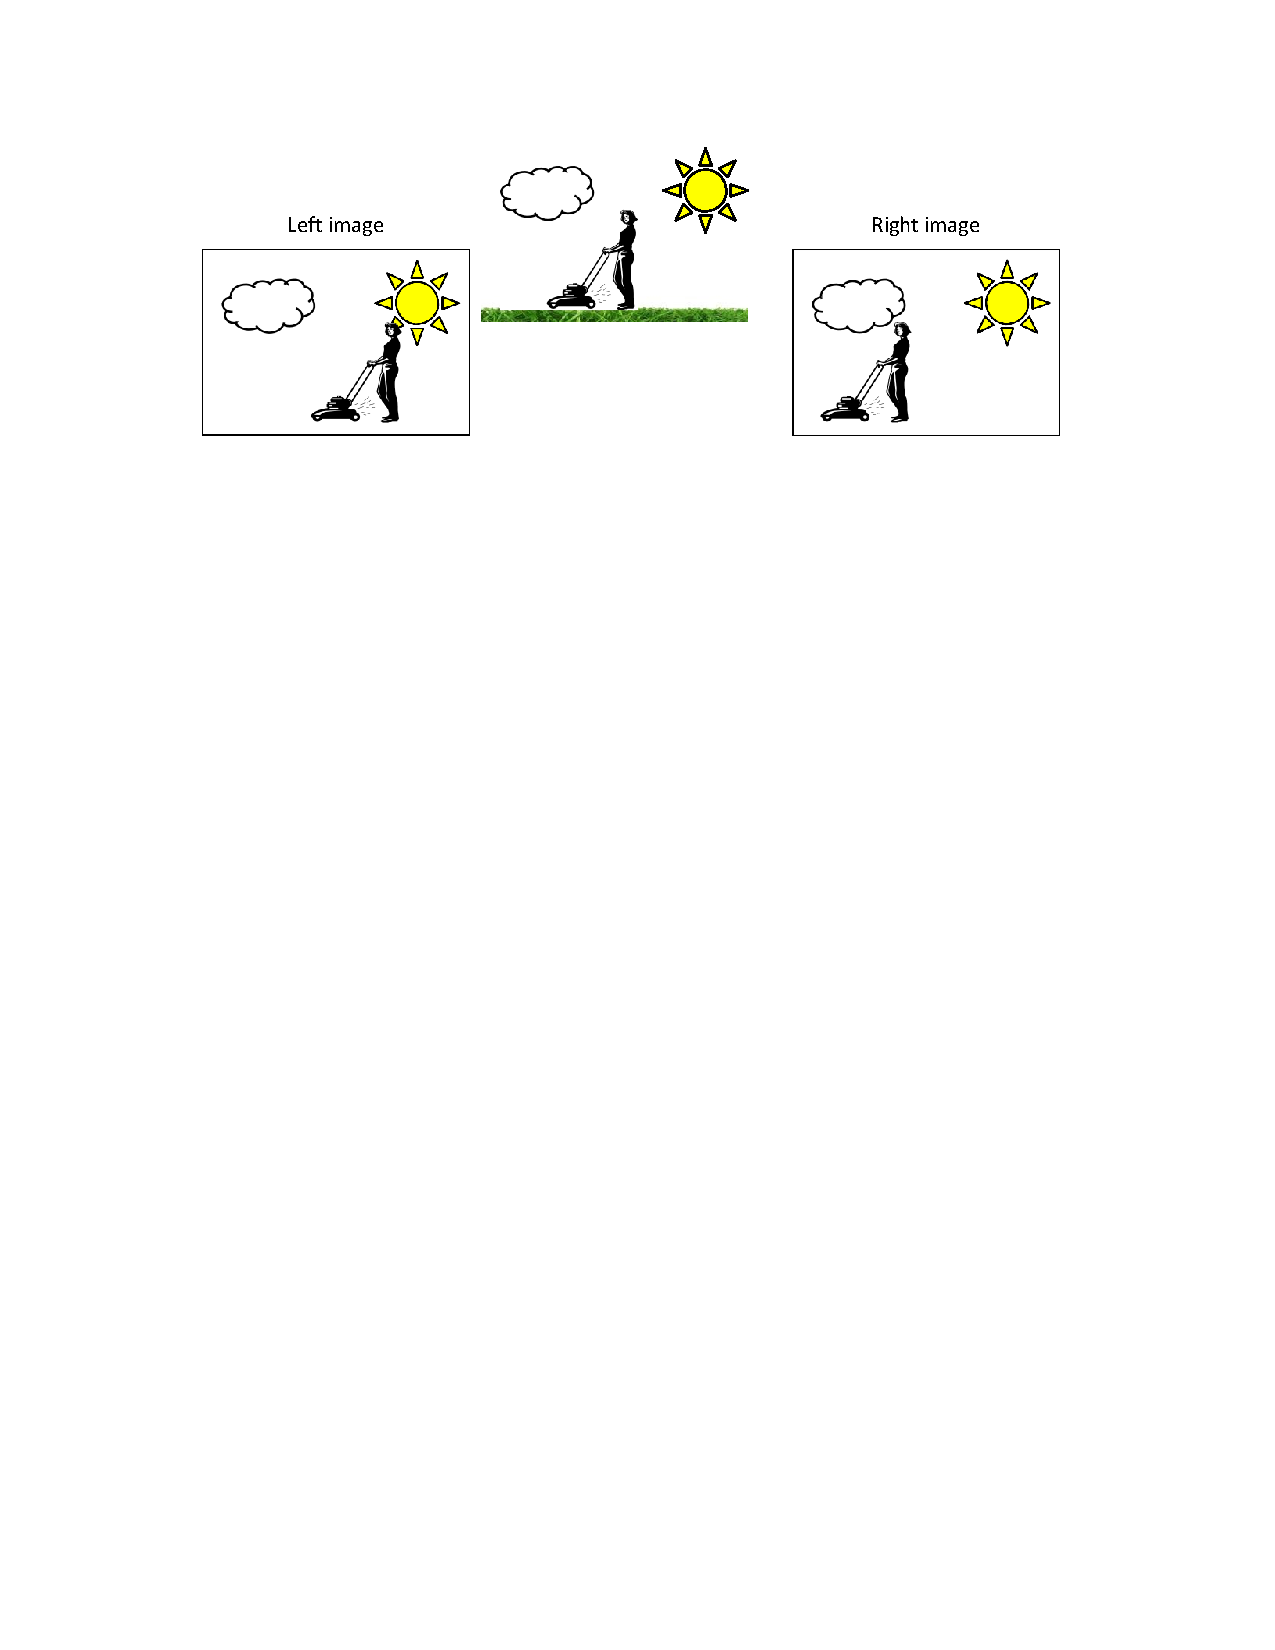
\includegraphics[width= 3 in]{LIRI.pdf}
\end{center}
\caption{The principle of stereoscopic images} \label{tdof}
\item{Objects close to the camera will be placed more to the right in the left image - and more to the left in the right image.}
\item{Faraway objects, such as the sun and the cloud, will be located at approximately the same position in both images.}
\end{figure}
\end{frame}
\begin{frame}
\frametitle{Introduction to Stereo matching or Stereo Vision problem}
\begin{itemize}
\item To find the matching pixel in left and right image for stereo pair image is known as \textbf{stereo vision, stereo correspondence or stereo matching.}
\item In stereo matching aim is to find the matching pixel for a stereo pair image as input image which consists of left and right image and result of finding matching pixel is saved as Depth map or disparity map.
\item The disparity is horizontal distance between two matching pixel and horizontal pixel distance for each pixel coordinates is nothing but Disparity map.

\end{itemize}
\end{frame}


\begin{frame}
\begin{figure}
 \frametitle{Introduction to Stereo matching or Stereo Vision problem}
  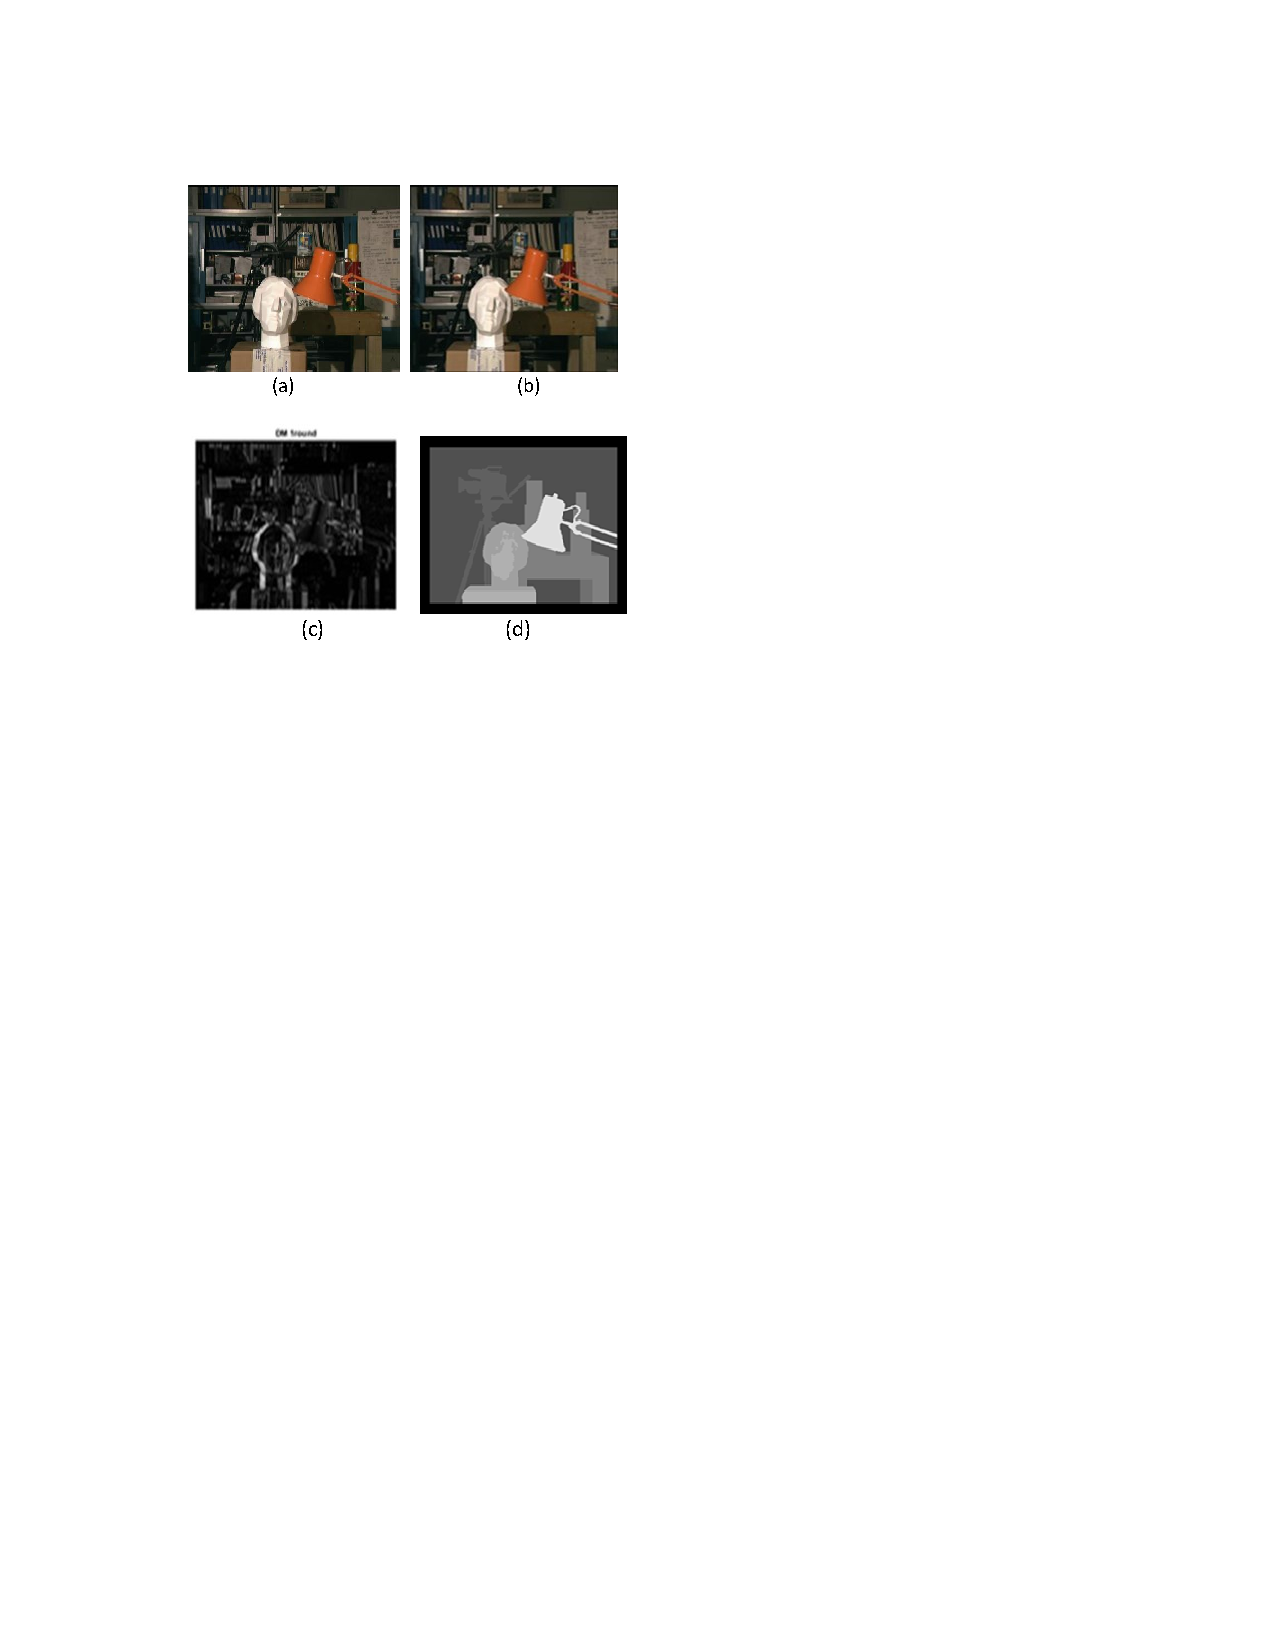
\includegraphics[width=2in]{4f.pdf}
  \caption{(a)Left Image (b)Right Image(c)Depth map by Global Method(d)Ground truth}\label{}
\end{figure}
\end{frame}

\begin{frame}
\begin{itemize}
\frametitle{Classification of Stereo algorithm}
\item{The stereo algorithms based on  intensity profile are \textbf{Area-based and Feature- based algorithm } }
\item{The constrains in area- based algorithm  is to find the optimal size of the window }
\item{The feature-based algorithms is restricted to using only specific feature,that only yield sparse disparity maps}
\item{Global algorithm are based on baysian approach finds disparity   as a energy minimization problem}
\item{Global stereo algorithm  are  \textbf{Graph cut and belief propagation}}
\end{itemize}
\end{frame}

\begin{frame}
\begin{itemize}
\frametitle{Applications of Depth Map or Disparity Map}
\item{View Interpolation can done using stereo pair and Depth map
\begin{figure}
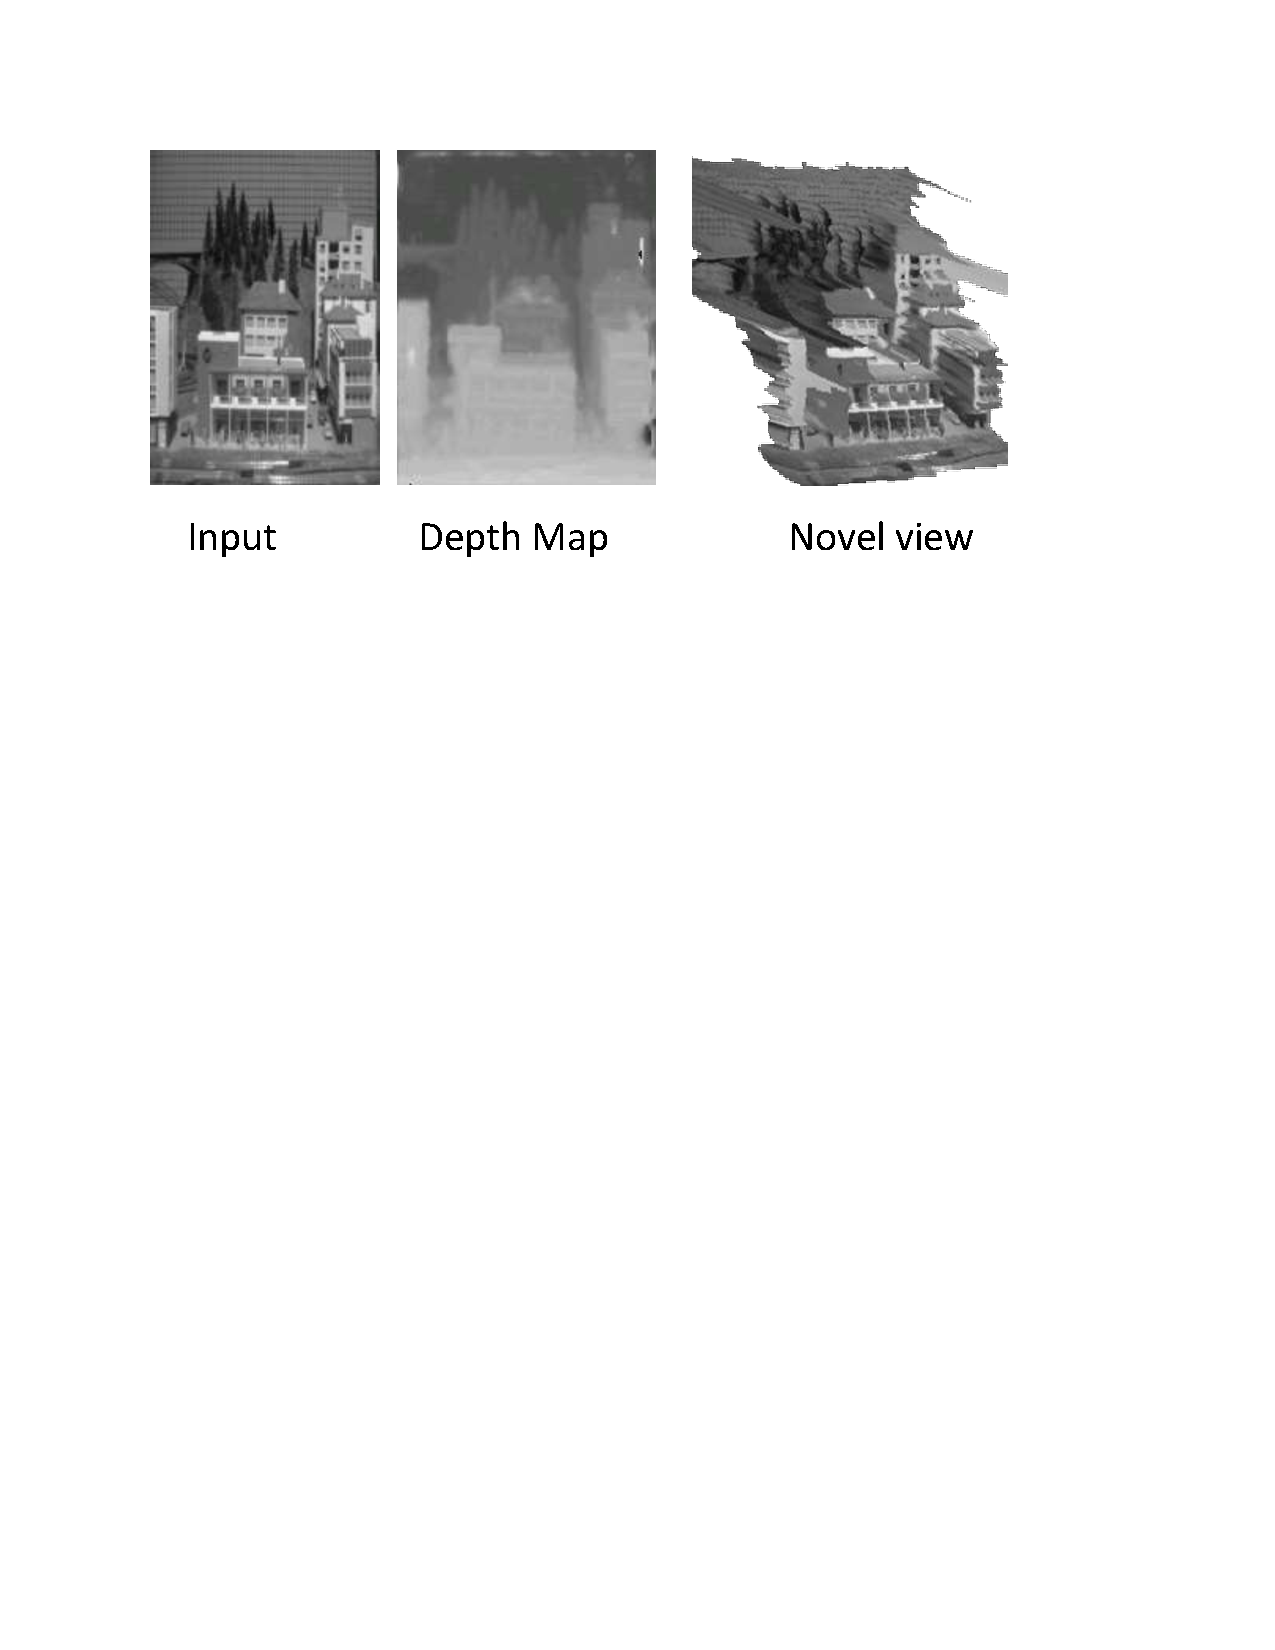
\includegraphics[width=2.5in]{interpola.pdf}
\end{figure}}
\item{Image sequence analysis in entertainment,information transfer and for reconstruct 3D model sequences
\begin{figure}
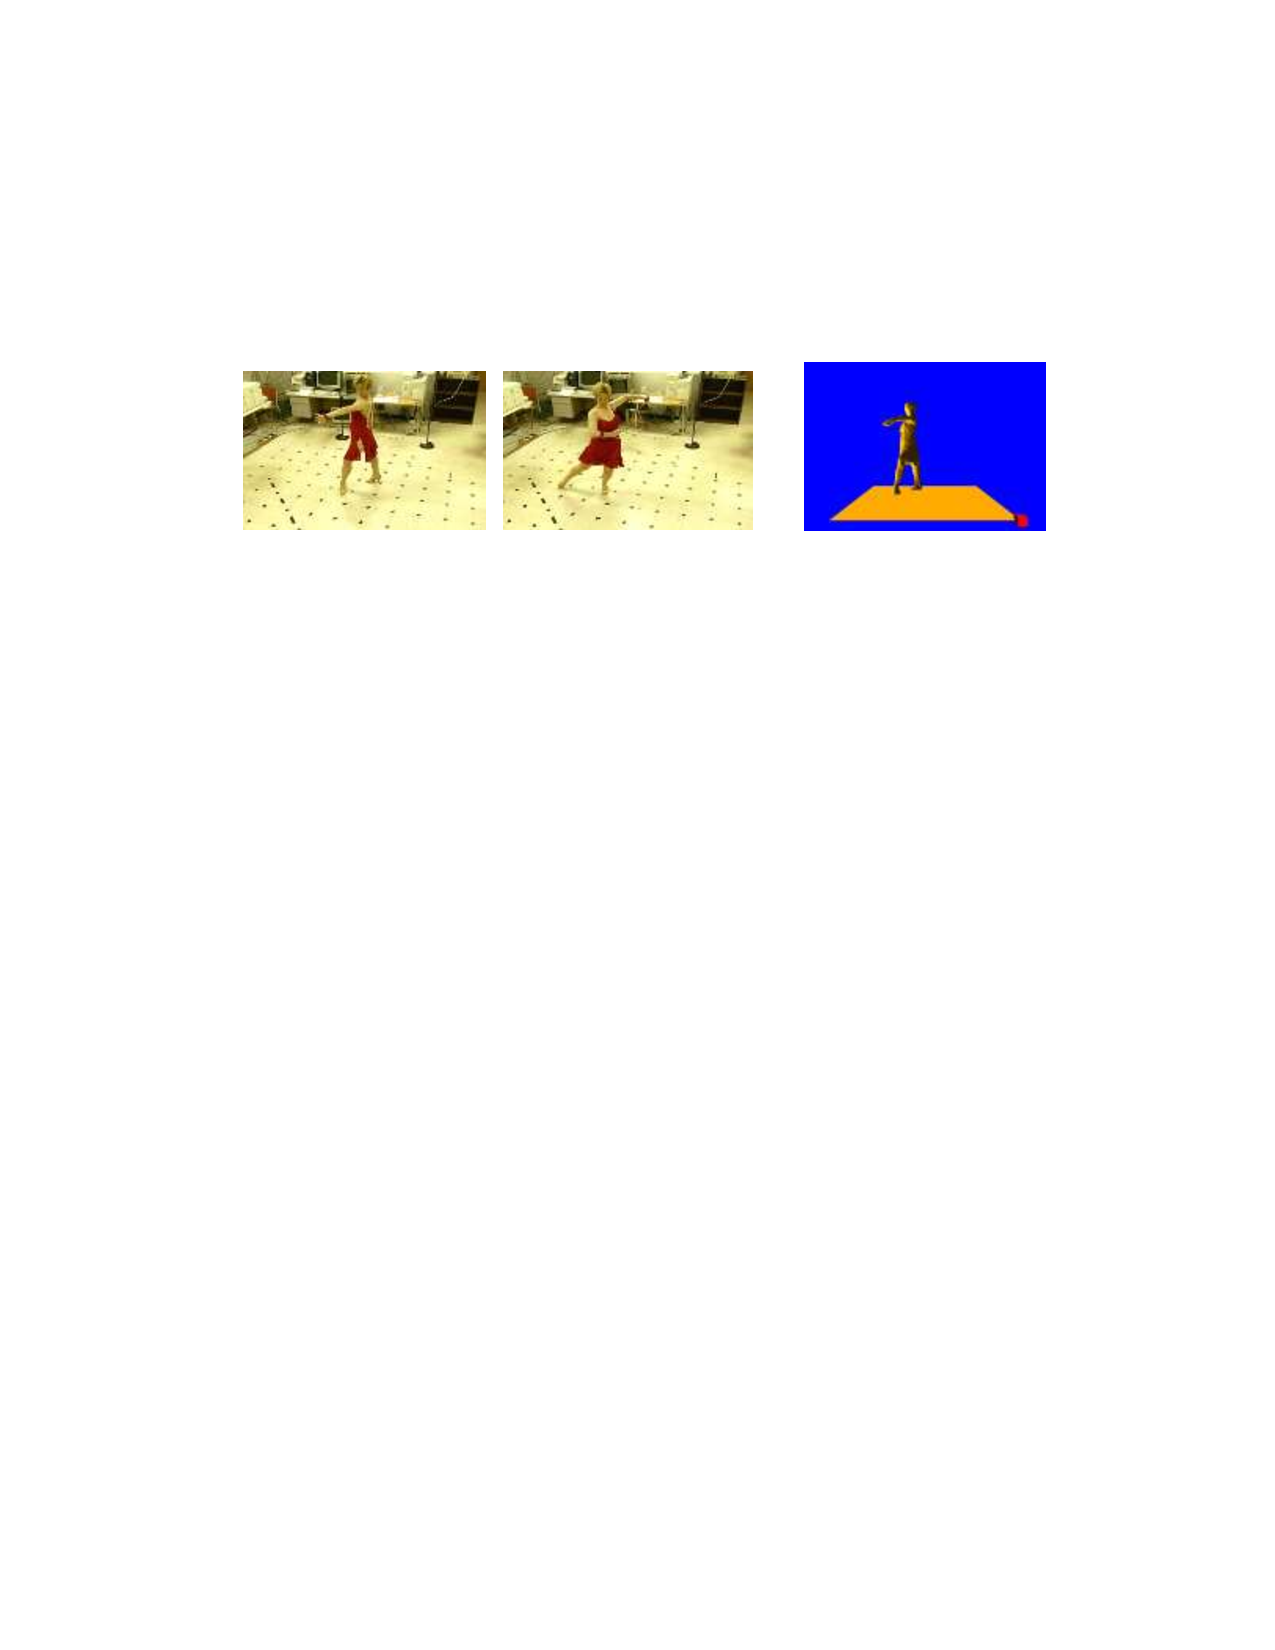
\includegraphics[width=2.5in]{3dmodel.pdf}
\end{figure}}
\end{itemize}
\end{frame}

\begin{frame}
\begin{itemize}
\frametitle{Applications of  Depth Map or Disparity Map}
\item{Used for robot navigation and depth information is used for object recognition to separate occluded image components
\begin{figure}
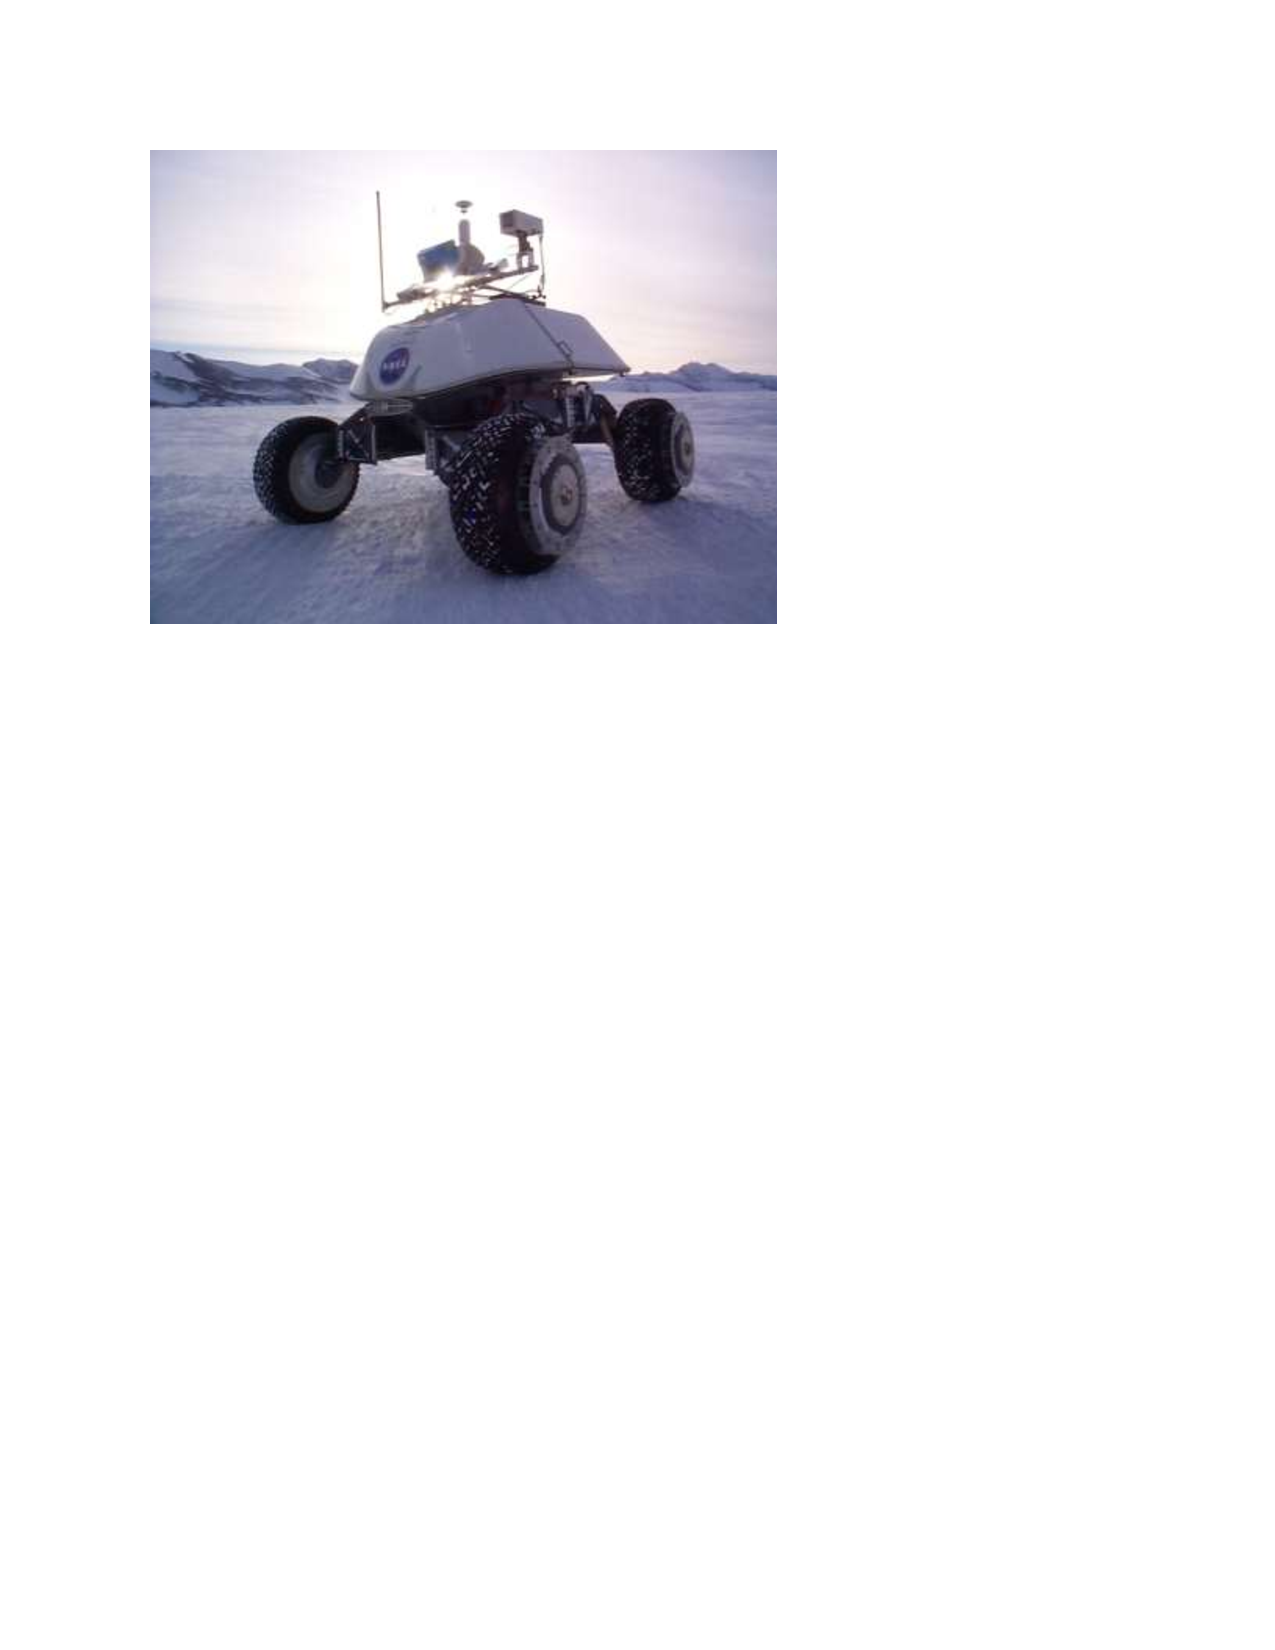
\includegraphics[width=1in]{robo.pdf}
\end{figure}}
\item{Scientific applications such as   extracts  information from aerial surveys and  for calculation of contour maps  }
\item{Gaze correction for video conferencing }
\end{itemize}
\end{frame}


%%Slide which includes table
%

%\begin{frame}
%\begin{itemize}
%\frametitle{Introduction to Stereo matching}
%\item{The disparity  is difference in image location of the same 3D point for 3D image,when projected under  two or more different cameras.}
%\item{The stereo image is captured by two cameras at two different view point of same scene or object.}
%\item{Two problems arises when finding disparity for stereo image.}They are
%\begin{enumerate}
%  \item {Use of  prior knowledge or camera calibration}
%  \item{Finding corresponding point in right image for each point in left image which known as \textbf{stereo vision problem ,stereo matching or stereo correspondence}.}
%\end{enumerate}
%\item{First problem can be solved by using projectile approach  known as epipolar geometry which uses properties of rays rather than intrinsic parameters of camera.}
%\end{itemize}
%\end{frame}
%
%\begin{frame}
%\frametitle{Introduction to Stereo matching}
%\begin{figure}
%\begin{center}
%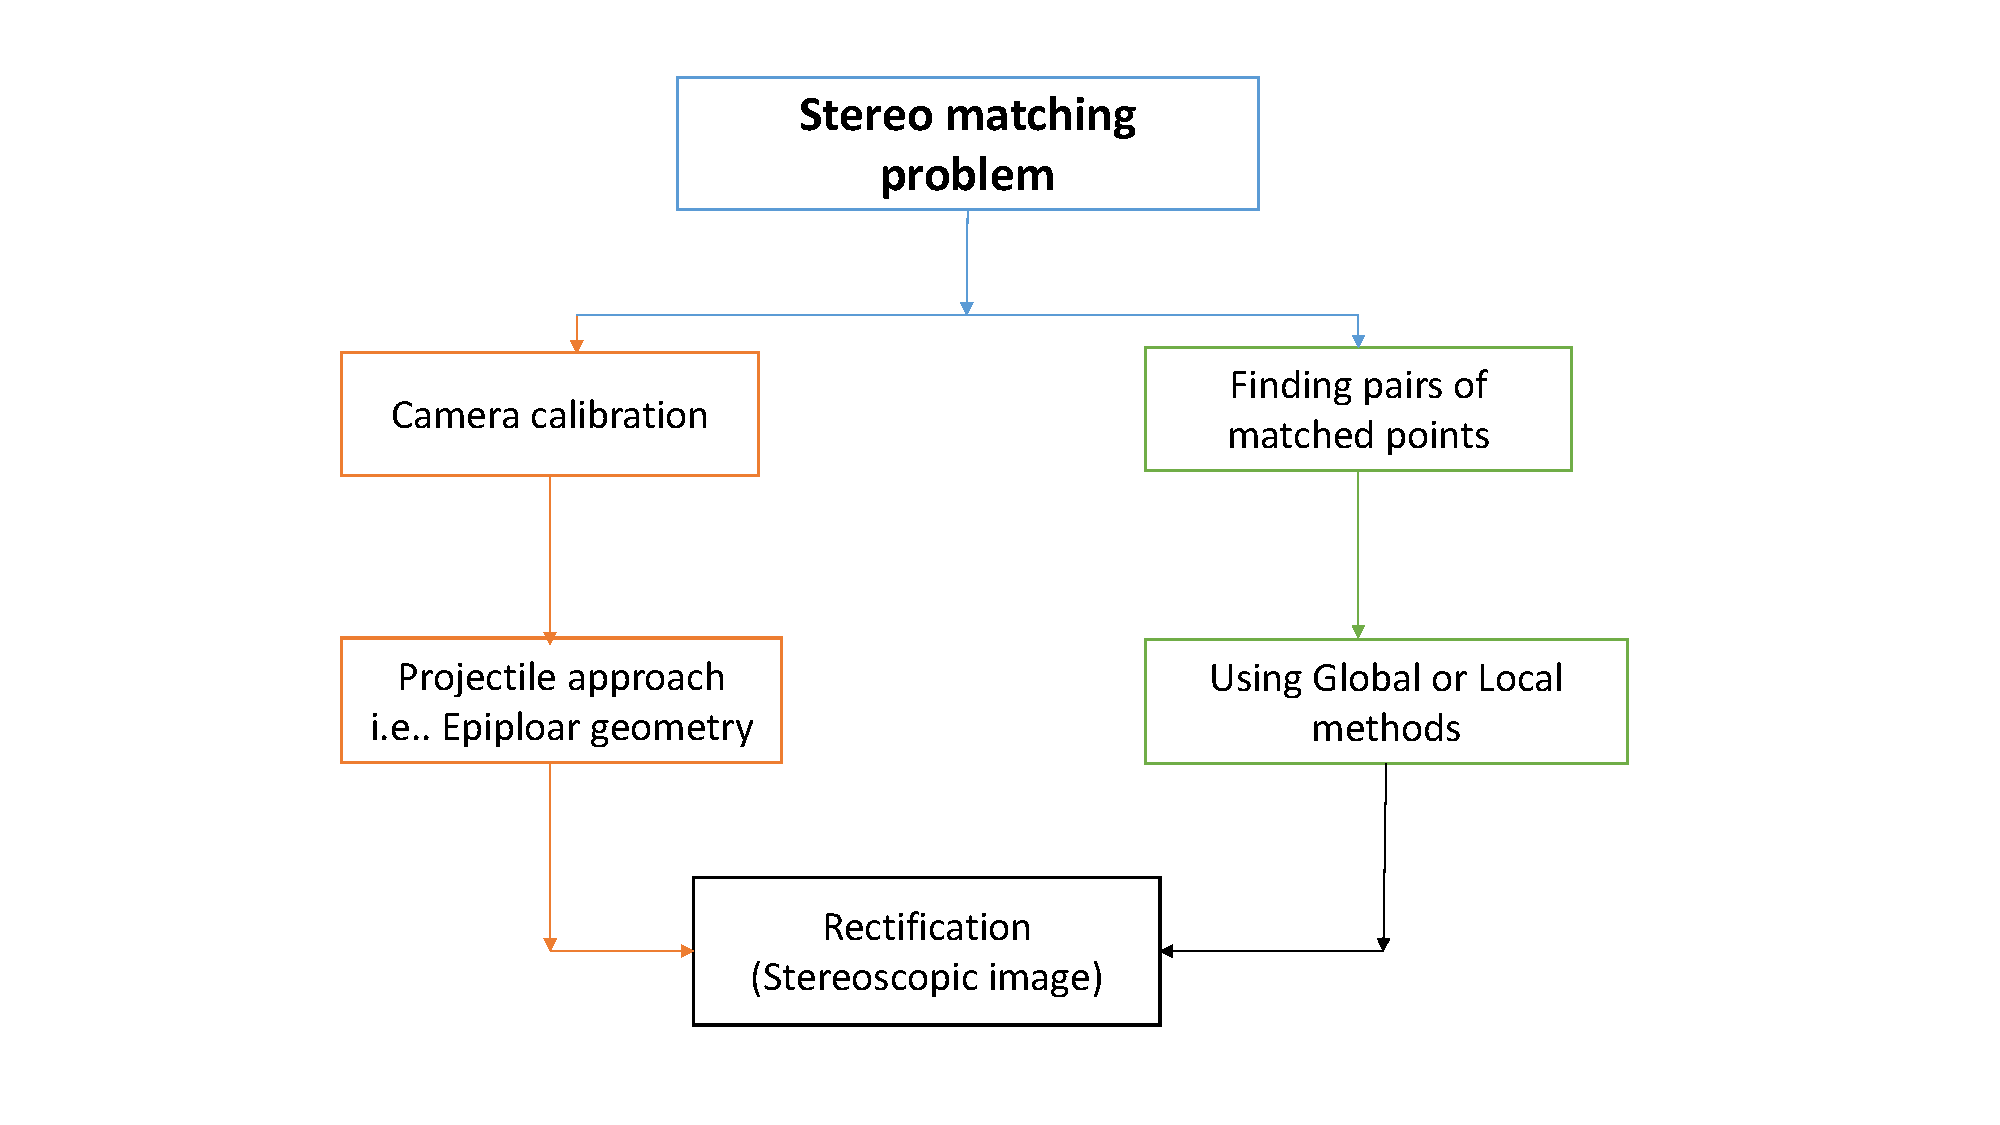
\includegraphics[width=5in]{stereomatching.pdf}
%\caption{Flow chart for stereo matching} \label{lined}
%\end{center}
%\end{figure}
%\end{frame}
%
%
%\begin{frame}
%\begin{itemize}
%\frametitle{Mathematical Representation of Global stereo Algorithm}
%\item{The stereo matching problem can be expressed as global function}
%\item{Stereo matching problem can be interpreted in terms of probability theory as well as markov network}
%\end{itemize}
%\end{frame}
\begin{frame}
\frametitle {Mathematical Representation of Stereo matching}

\begin{itemize}
\item{\textcolor[rgb]{0.00,0.50,1.00}{\emph{The stereo matching problem can be expressed  in terms of Markov}}}
\item {The markov network model is a probability graphical model which consists of undirected graph of 'n' nodes with pair wise potentials as compatibility function}
\item{ Y is evidence or observed state node,$X\_s$ is hidden node state,state of each nodes  $'i'$ represent as \textbf{X}\_i for given evidence,To find most likely set of nodes $\{X\_1, X\_2, X\_n\}$ for given evidence 'Y' and compatibility between neighboring nodes can be expressed as a joint probability distribution function of $n$ nodes. }
\item
\begin{description}
 P (X\_1, X\_2, X\_n/Y) =$\prod \limits_{All nodes \textbf{s}}\Phi(X\_s ,Y )$$ \prod\limits_{(All neighboring of nodes \textbf{s,t})}\Phi(X\_s ,X\_t )$
\end{description}
\end{itemize}
\end{frame}



\begin{frame}
\frametitle {Mathematical Representation of Stereo matching}
\begin{itemize}
\item{\textcolor[rgb]{0.00,0.00,1.00}{\texttt{The stereo matching problem can be expressed  in terms of probability theory}}}
\item{Markov network model is analogous to Bays theorem }
\item {According to Bays theorem :P(X/Y) = P(Y/X)*P(X)/P(Y)}
\item{Y is stereo set and X is disparity map,$P(Y)$ =1(assumption)}
\item{The disparity map can be obtained by maximizing probability of disparity map to stereo set i.e.$P(X/Y)$ and probability  can be expressed in terms of Datacost  and smoothness cost functions}

\end{itemize}
\end{frame}







\begin{frame}
\frametitle{Mathematical Representation of  stereo Algorithm}
\begin{table}
  \centering
  \caption{\texttt{Stereo matching problem as probability theory and markov network}}
\begin{tabular}{|c|c|c|}
  \hline
  % after \\: \hline or \cline{col1-col2} \cline{col3-col4} ...
   S.No& Markov network & Probability Theory\\\hline
 1 &  Maximizing joint & Maximizing probability    \\
     & probability     & of disparity map   \\
      & distribution        & to stereo set \\
      & i.e$P(X_1 ,X_2,�..X_n/Y)$        & i.e. $P(X/Y)$          \\ \hline
 2 & Markov state    & Set of pixels in   \\
       &            & with assigned  disparity value   \\ \hline
 3& For given Evidence Y & For given set of stereo images\\ \hline


\end{tabular}
\end{table}
\end{frame}




\begin{frame}
\frametitle{Mathematical Representation of  Stereo Algorithm}
\begin{itemize}
\item{To find Maximum A Posteriori (MAP) estimation in markov network is NP hard means to get a solution for such problem takes unthinkably long time
 because each pixel (node) in disparity map can take any value in disparity space (state)}
\item{For example for Tsukuba image of size 384 x 288=110592 pixel with 16 disparity levels gives $16 ^{110592}$ combinations,So it is difficult to find solution }
\item{Belief Propagation algorithm is approximate solution to estimate Maximum a Posteriori (MAP) in reasonable amount of time}
\end{itemize}
\end{frame}


\begin{frame}
\frametitle {Model used for Stereo algorithm}
\begin{itemize}
\item{The probability of stereo set to disparity map .i.e. P(Y/X) and the probability of disparity map i.e. P(X) is expressed as matching cost term and smoothness cost term.}
\item{The data cost   is based on the intensity differences between the two pixels. The Sum of Absolute Difference (ABS) or Sum of Square Difference (SSD) functions are used as data cost}
\item{smoothness cost models are Pott's model, linear and quadratic models}
\item{The Pott's model is a binary penalizing function with a single tunable  variable. This value controls how much smoothing is applied.}
\item{The linear and quadratic models have an extra parameter K. K is a truncation value that caps the maximum penalty.}
\end{itemize}
\end{frame}


\begin{frame}
\frametitle {Model used for Stereo algorithm :Pott's model, Linear and Quadratic models}
\begin{figure}
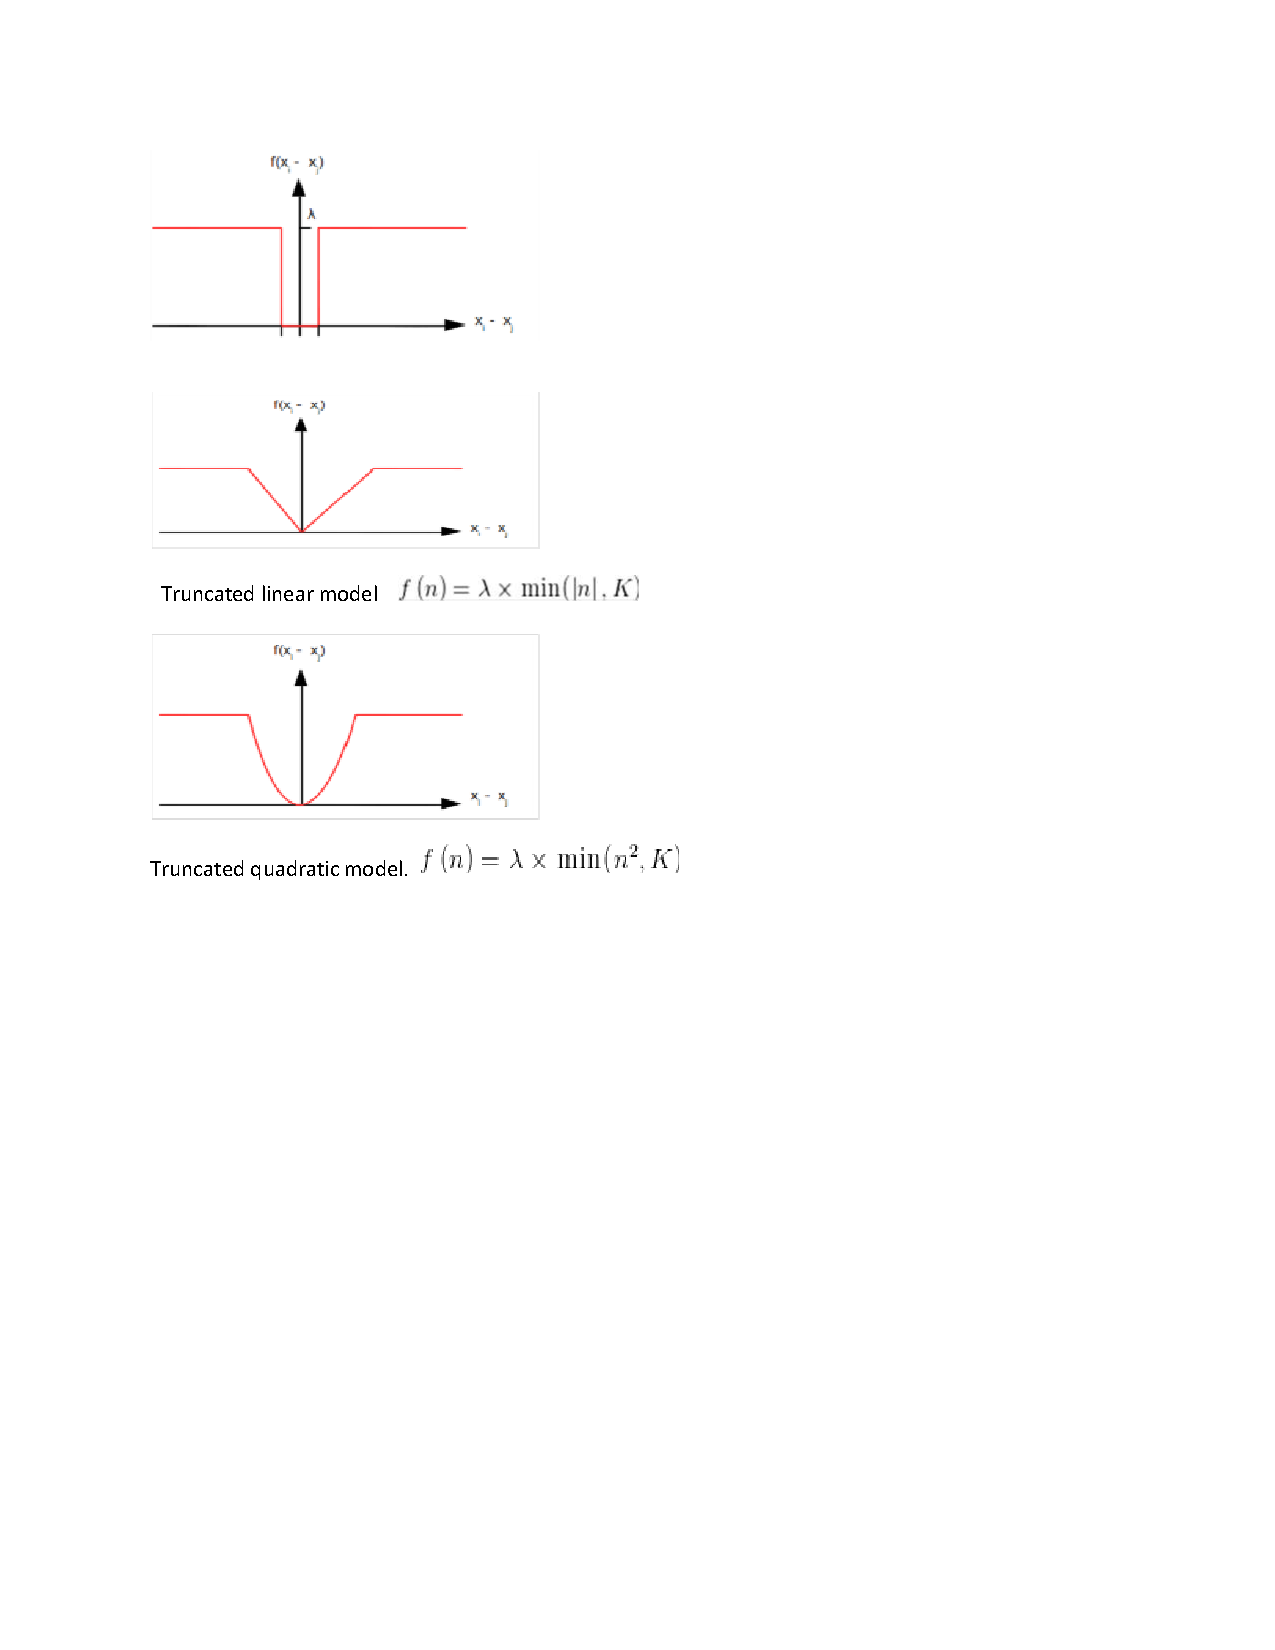
\includegraphics[width=2in]{SM.pdf}
\caption{Pott's model, Linear and Quadratic models} \label{lined}
\end{figure}
\end{frame}

\begin{frame}
\frametitle{Belief Propagation (BP) Algorithm}
\begin{itemize}
\item{The belief propagation algorithm was proposed by Pearl in 1988 for finding exact marginal's on graphs known as trees that contain no loops.It can be applied to graphs with loops also}
\item{The Loopy belief propagation is an approximate inference algorithm which keep passing the messages around markov state or node until stable belief state is reached,It is iterative algorithm, messages will converge on doing iterations.}
 \item{There are three main steps finding Maximum a Posteriori (MAP) estimation or beliefs in Belief Propagation algorithm}
\begin{enumerate}
  \item 	Normalization
  \item 	Message update or generation
  \item  	Finding belief
\end{enumerate}
\end{itemize}
\end{frame}
\begin{frame}
\frametitle {Belief Propagation (BP) Algorithm}
\begin{figure}
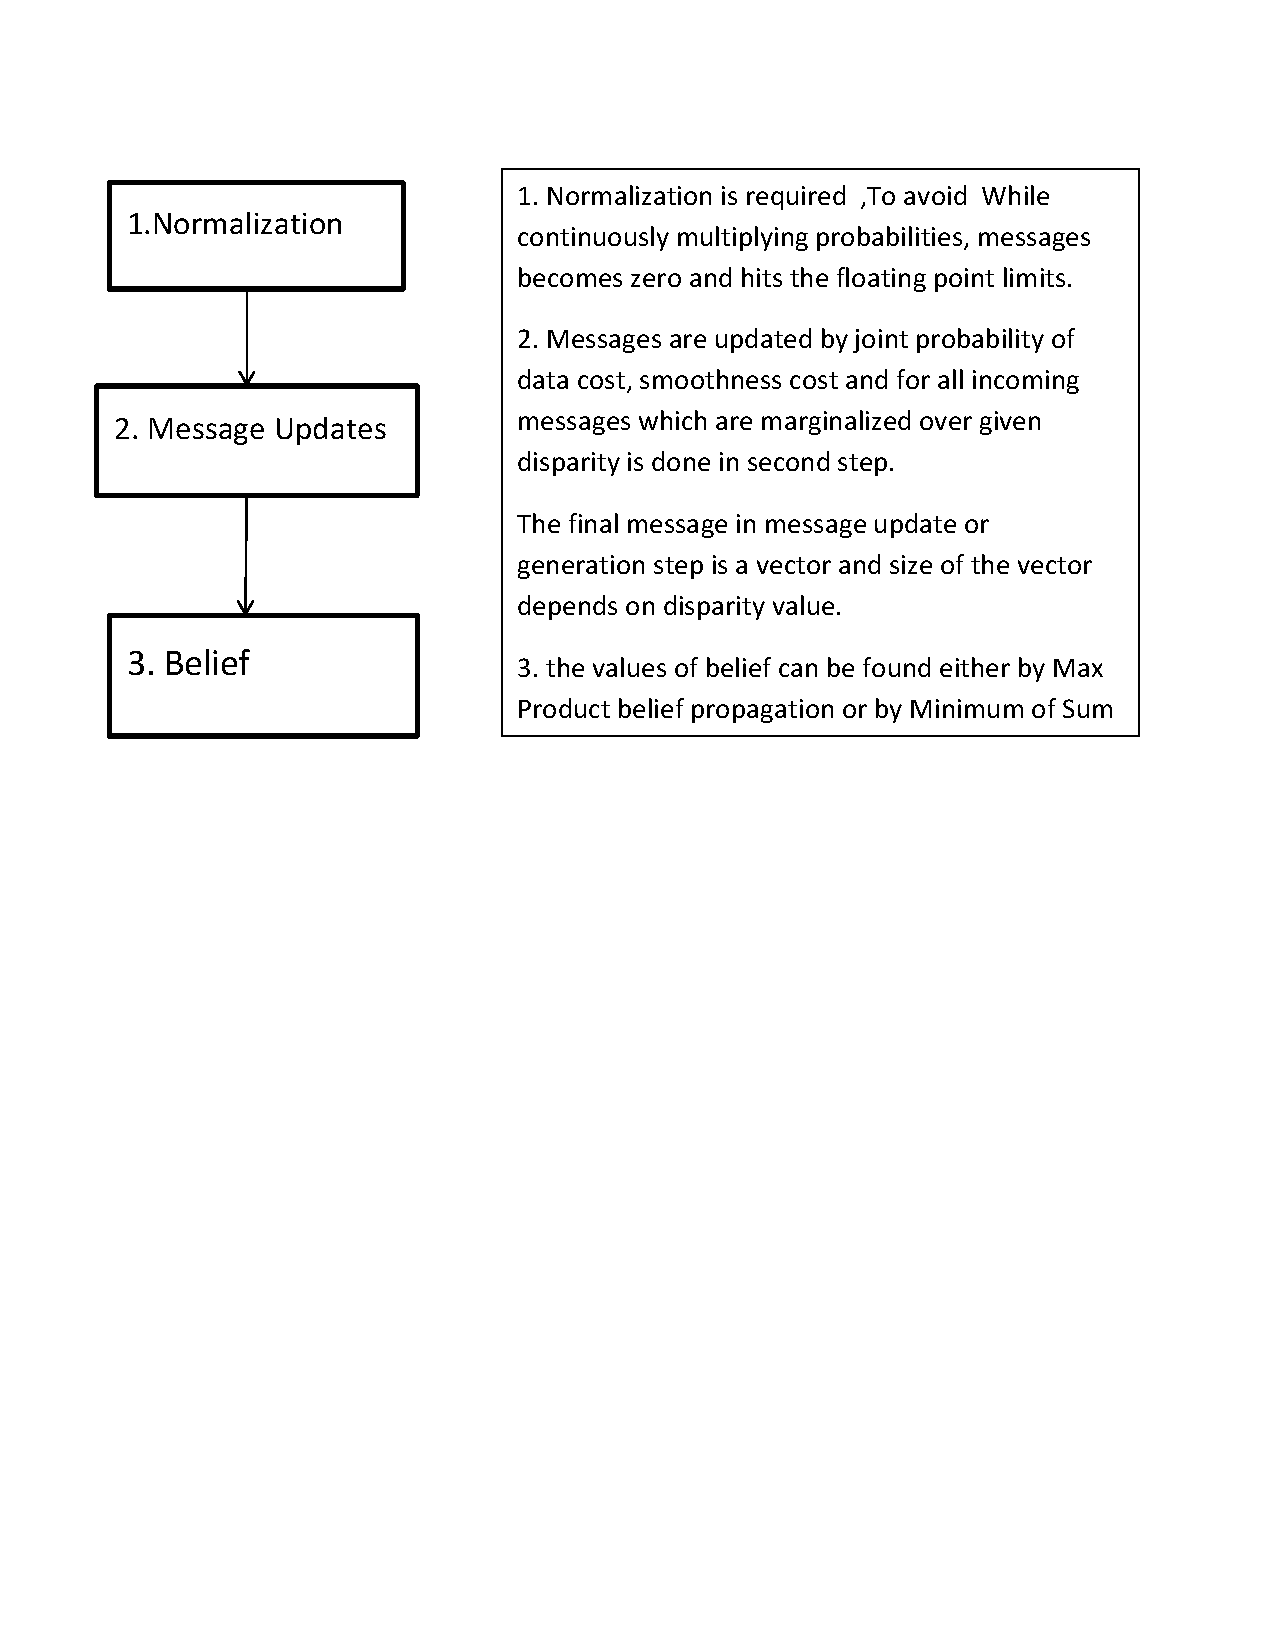
\includegraphics[width=4in]{stepbp.pdf}
\caption{Steps in BP algorithm} \label{lined}
\end{figure}
\end{frame}

\begin{frame}
\begin{itemize}
\frametitle{Implementation of BP Algorithm}
\item{ Block diagram for implementation of Global Stereo Algorithm using Belief Propagation\begin{figure}
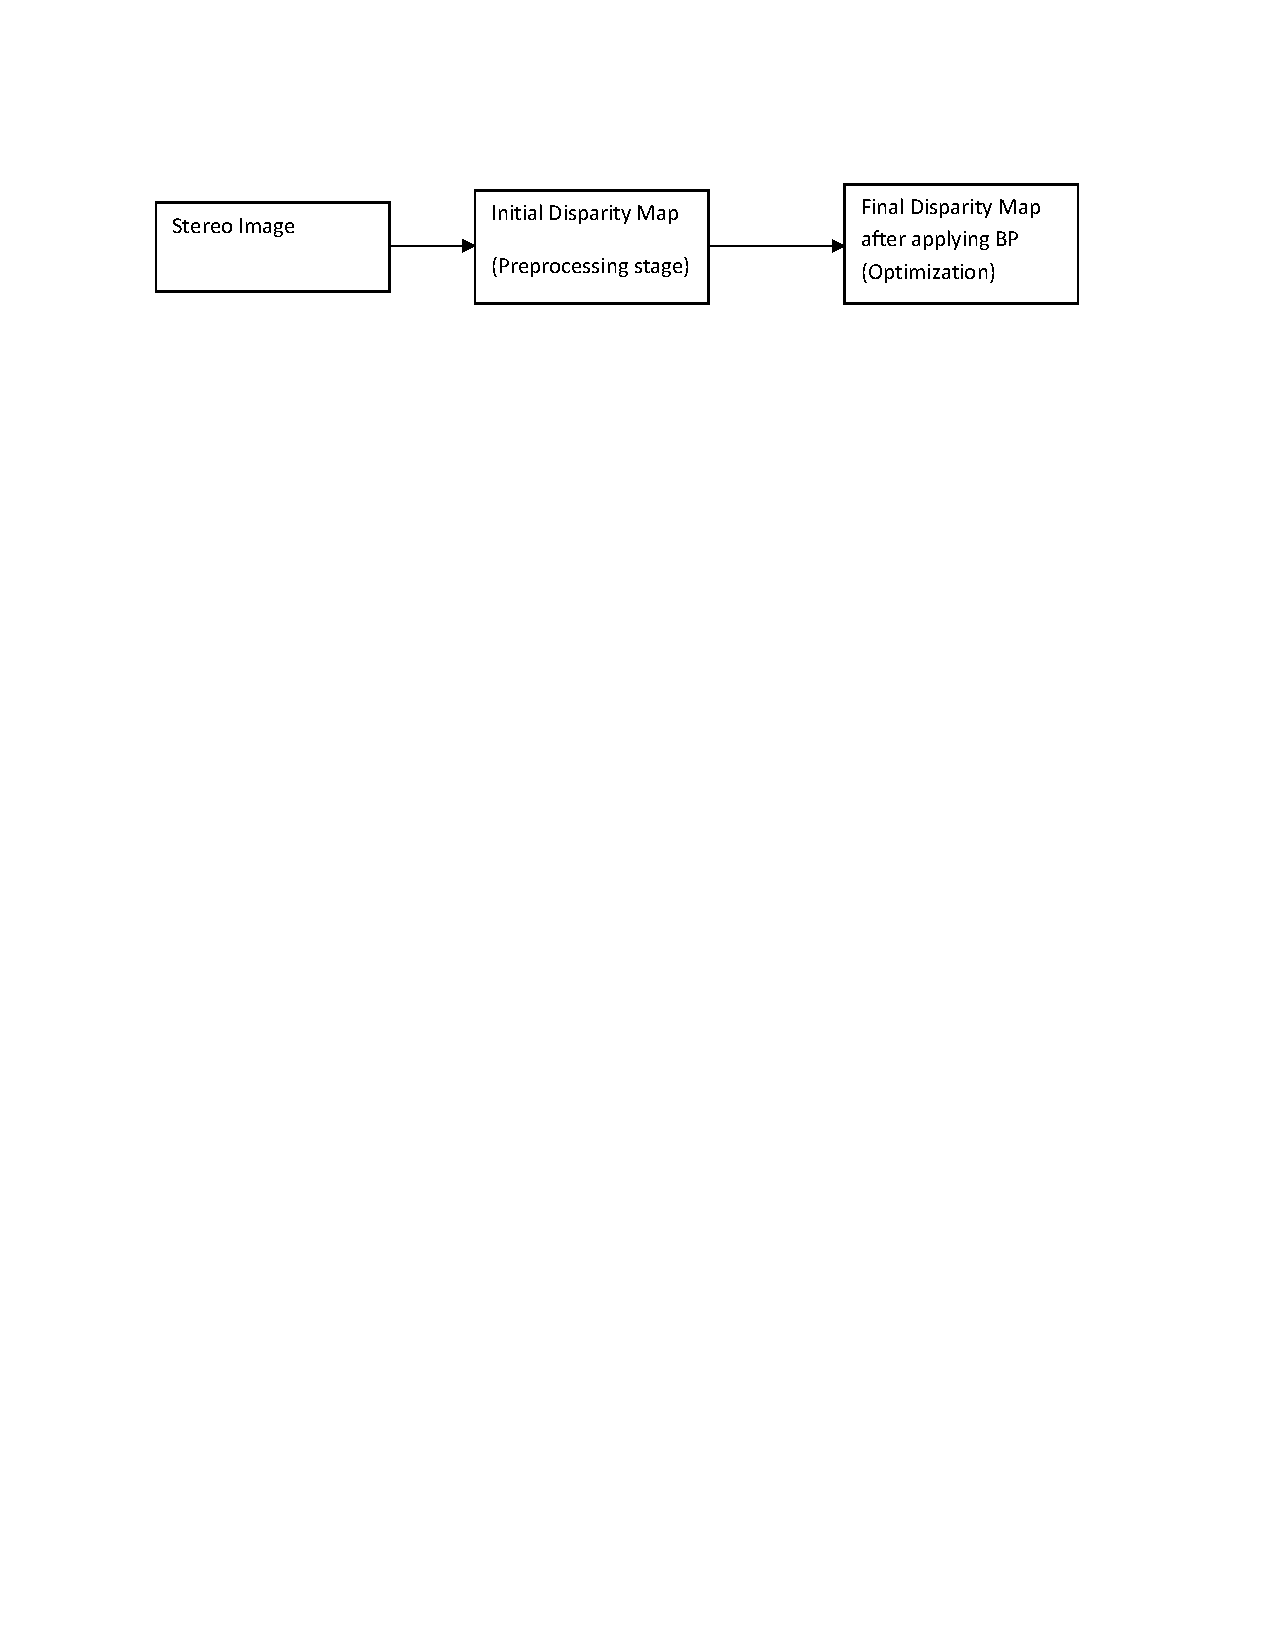
\includegraphics[width=4in]{bk.pdf}
\end{figure}}
\item {Stereo images(Rectified images) are taken as input}
\item{The software used for simulation is MATLAB version 2015}
\item{The  stereo images for testing are from  data sets of Middlebury computer vision web site (vision.middlebury.edu).}
\end{itemize}
\end{frame}

\begin{frame}
\begin{itemize}
\frametitle{Implementation of BP Algorithm}
\item{To find  Initial depth map  as a preprocessing  stage two methods are used.}
\item{First one is using MATLAB inbuild function "DisparityMap"in computer vision toolbox }
\item{Second method is minimum index method  by using sum of absolute difference function}
\item{Initial depth map generated by both methods are optimized by  Belief Propagation algorithm }
\end{itemize}
\end{frame}
\begin{frame}
\frametitle{Implementation of BP Algorithm:Results}
\begin{figure}

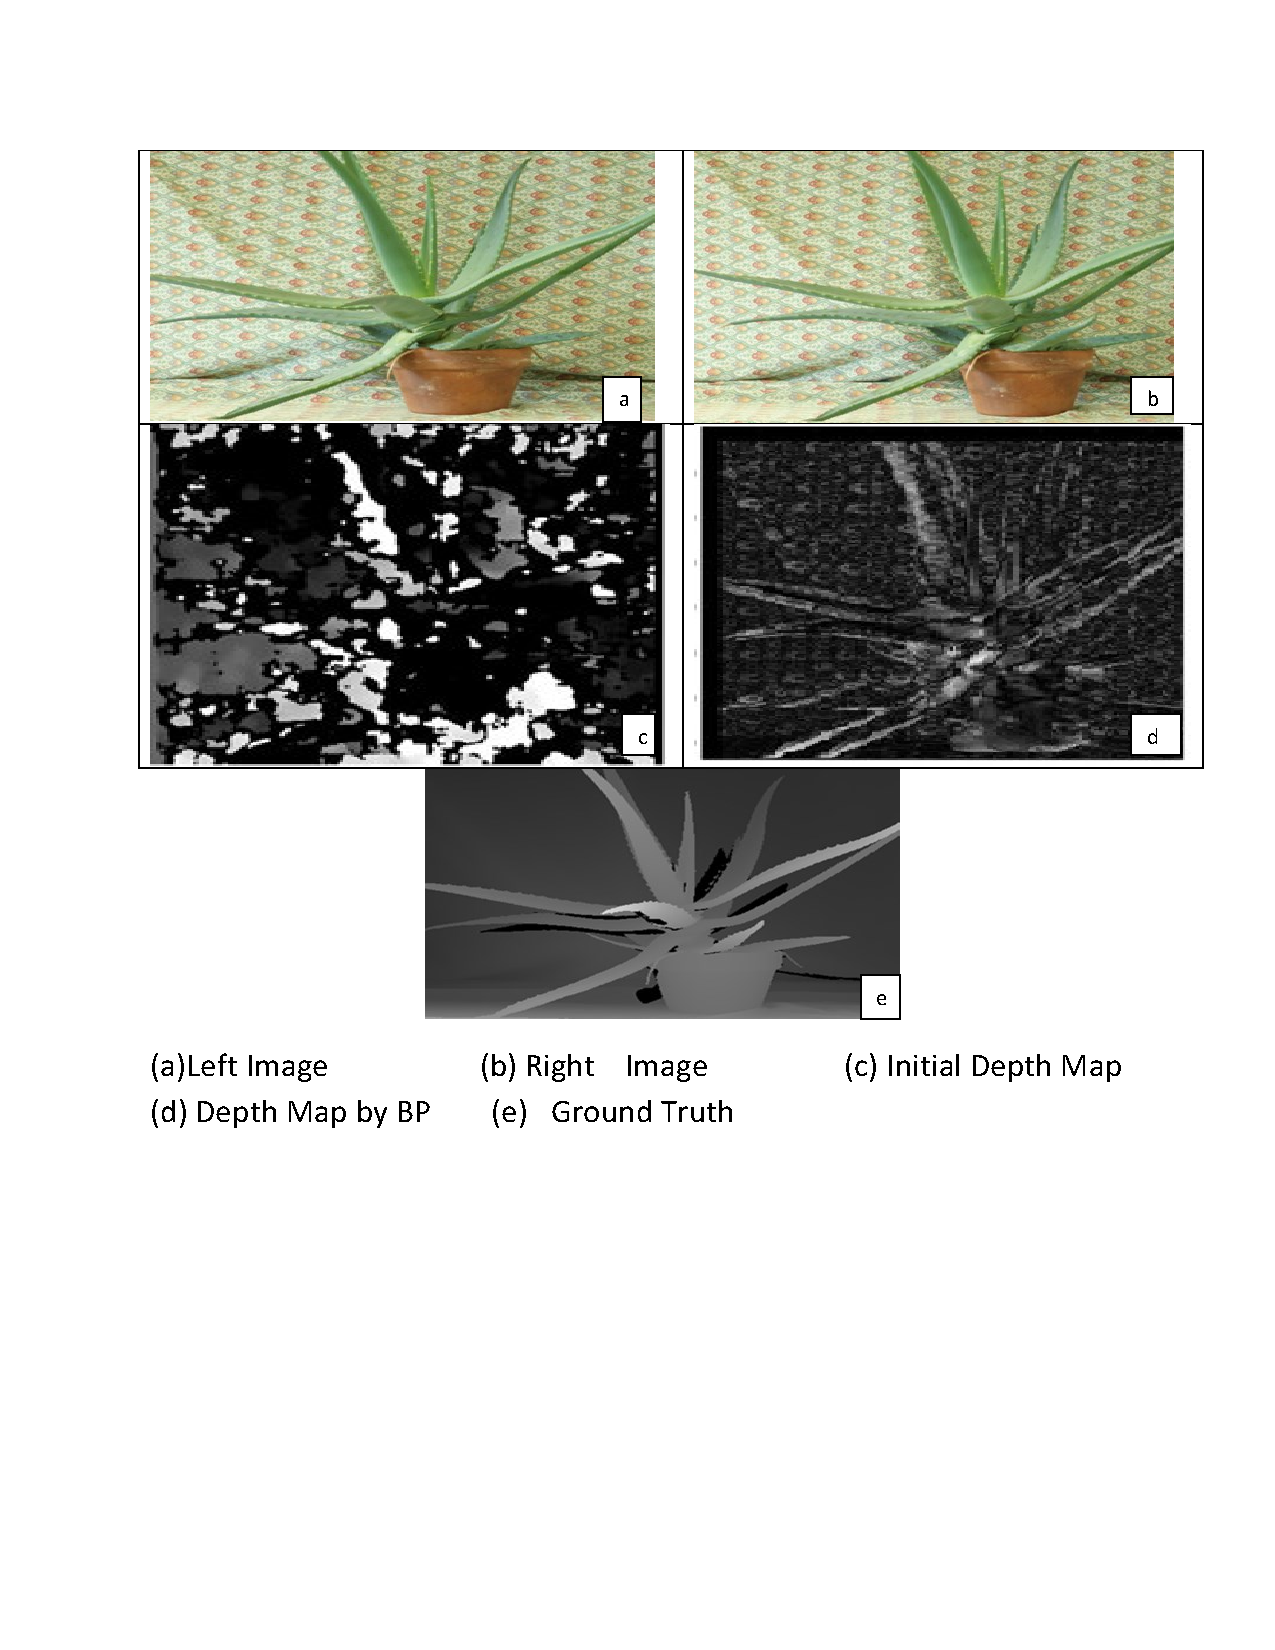
\includegraphics[width=3in]{alemat.pdf}
\caption{Representation of pot stereo image,Initial D.M by MATLAB function and it's depth map}\label{}
\end{figure}
\end{frame}


\begin{frame}
\frametitle{Implementation of BP Algorithm:Results}
\begin{figure}
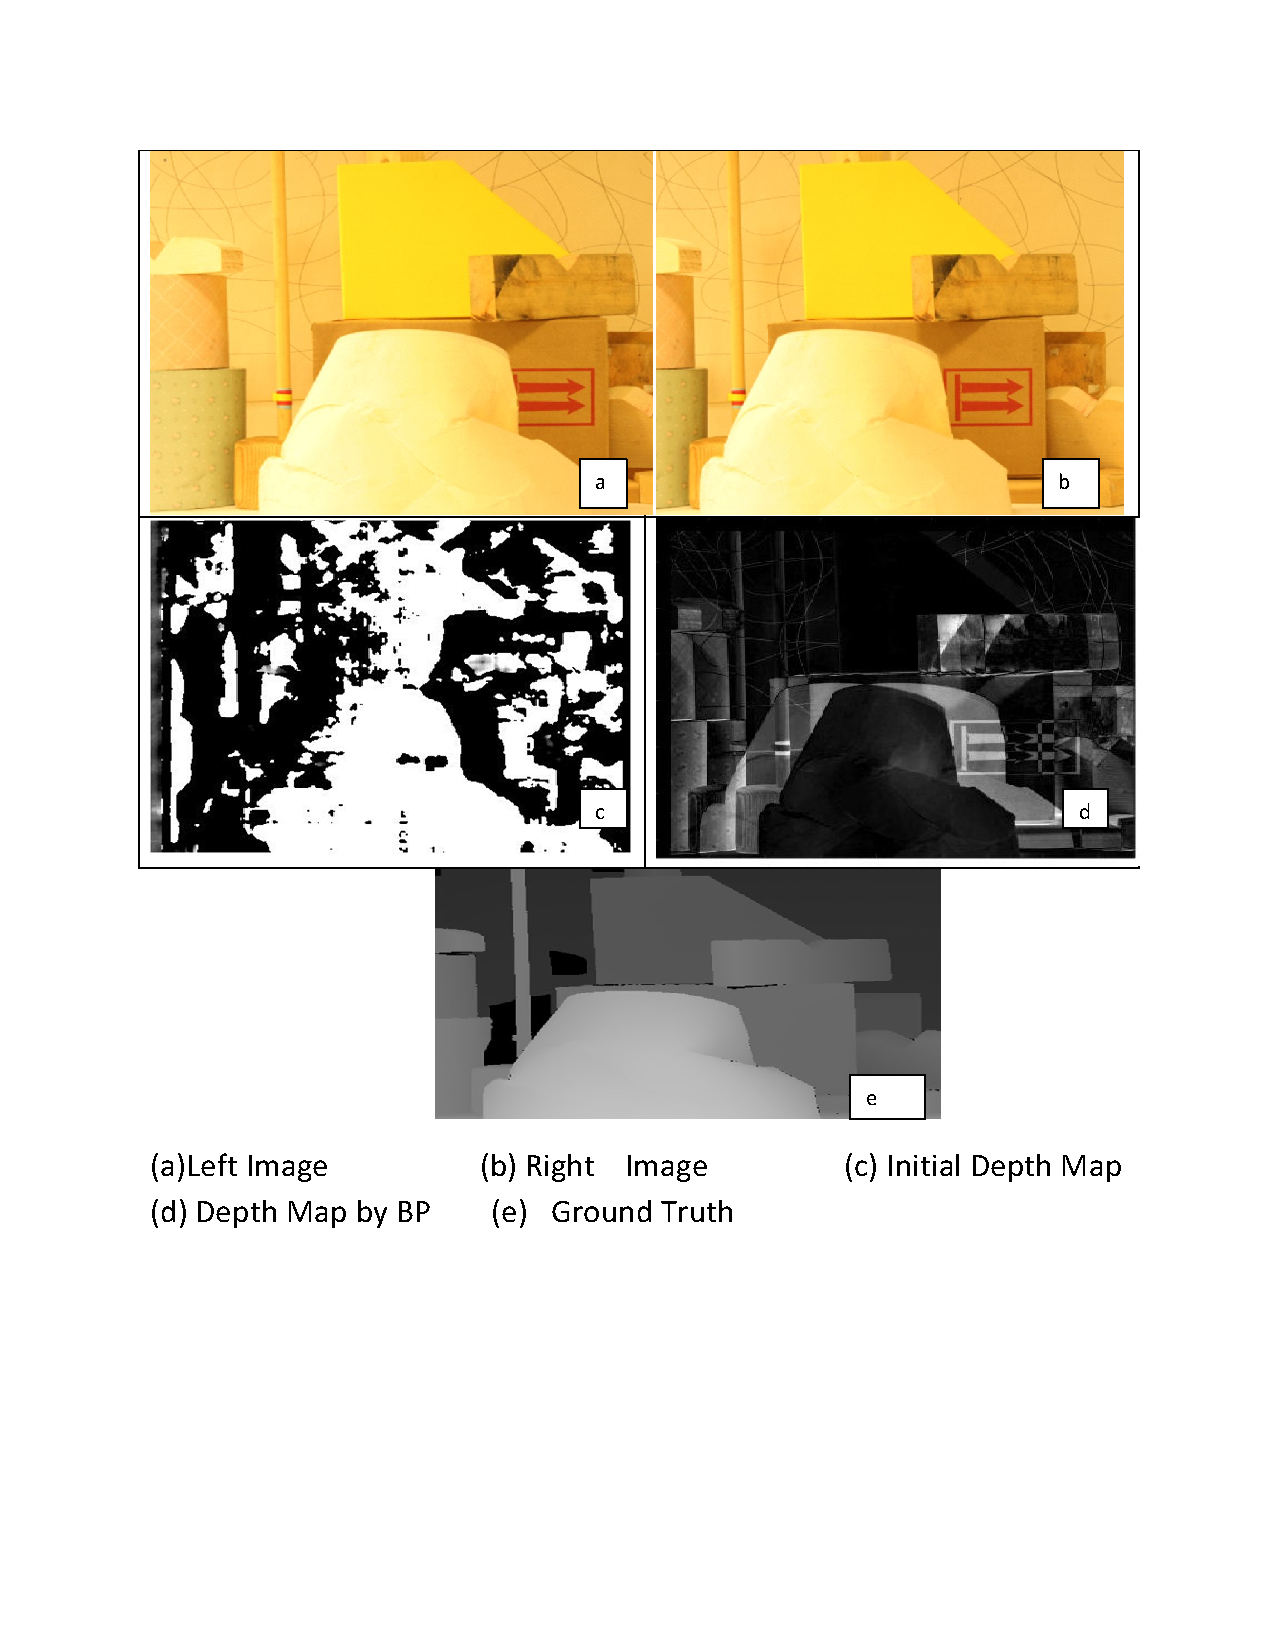
\includegraphics[width=2.5in]{potma.pdf}
\caption{Representation of pot stereo image,Initial D.M by MATLAB function and it's depth map}\label{}
\end{figure}
\end{frame}


\begin{frame}
\frametitle{Implementation of BP Algorithm:Results}
\begin{figure}
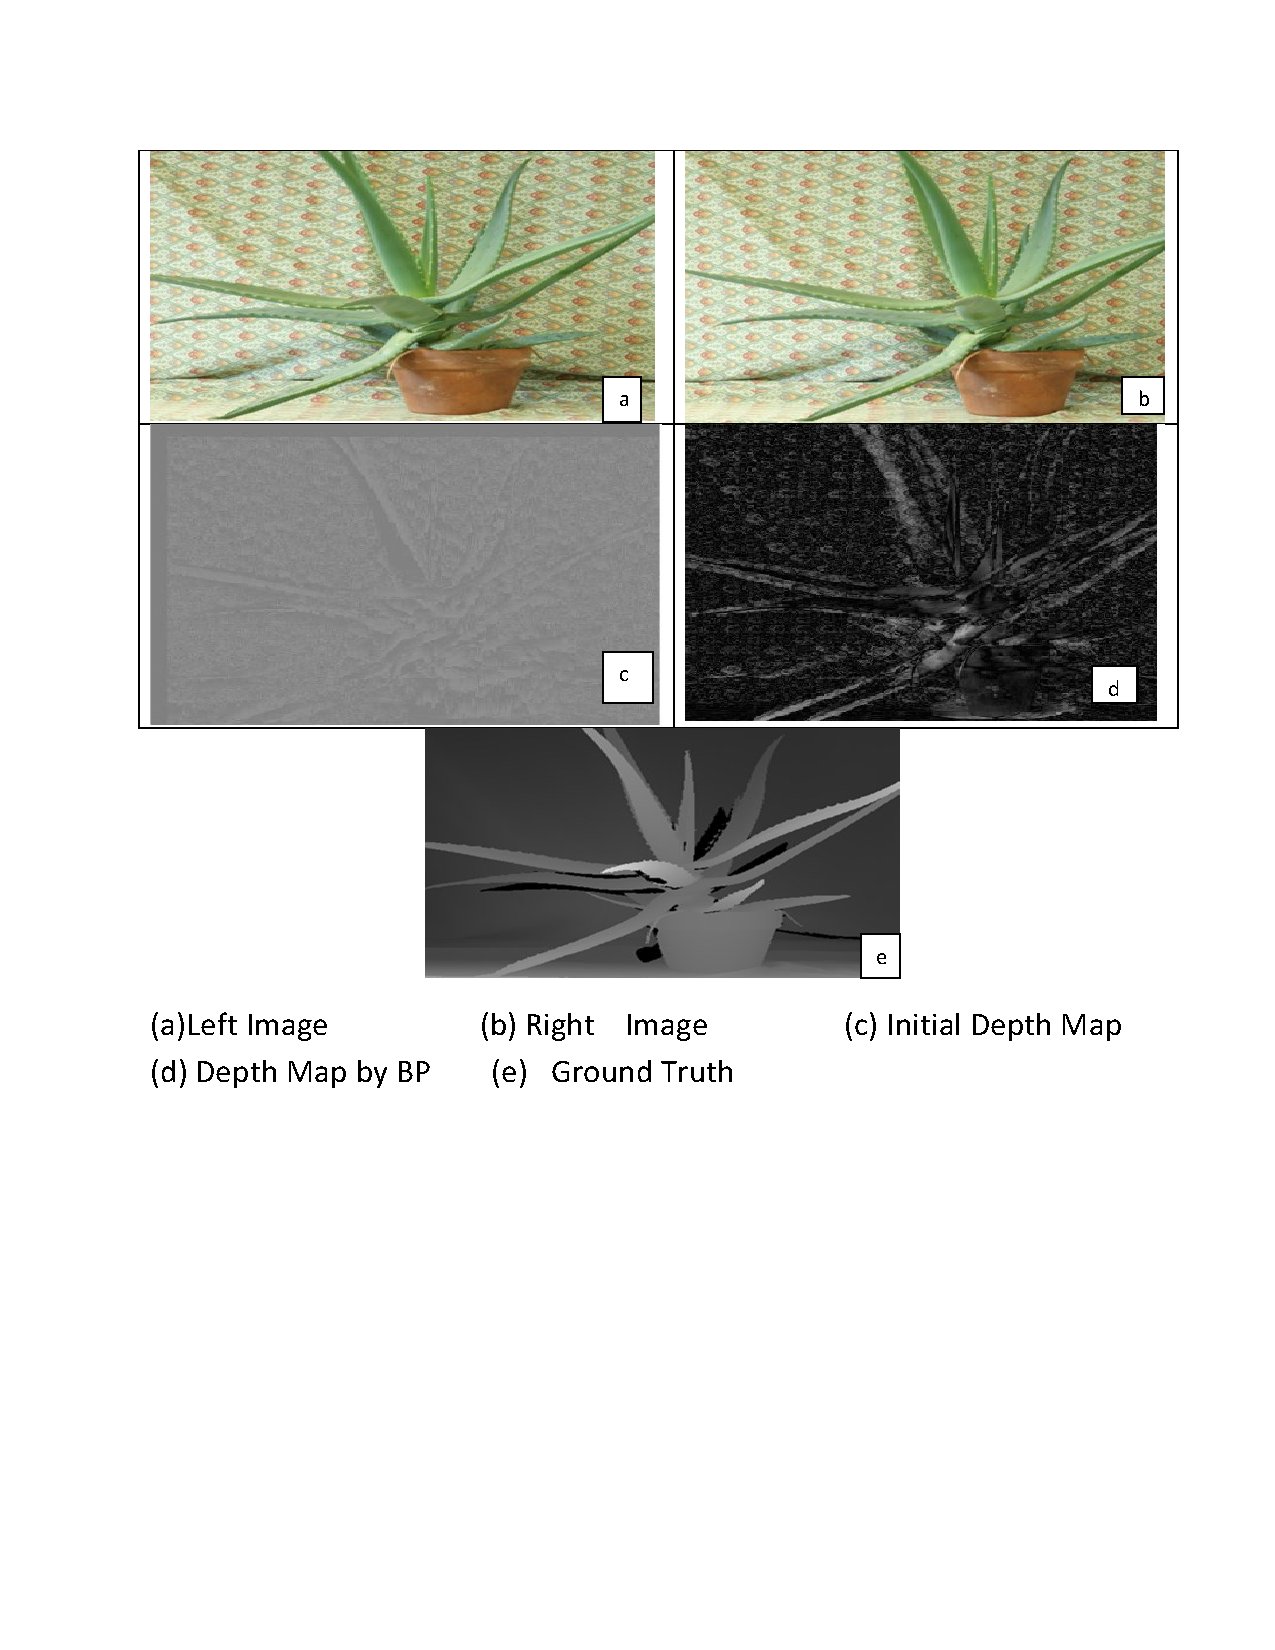
\includegraphics[width=3in]{alemi.pdf}
\caption{Representation of plant stereo image Initial D.M by Minimum Index method and it's depth map}\label{}
\end{figure}
\end{frame}

\begin{frame}
\frametitle{Implementation of BP Algorithm:Results}
\begin{figure}
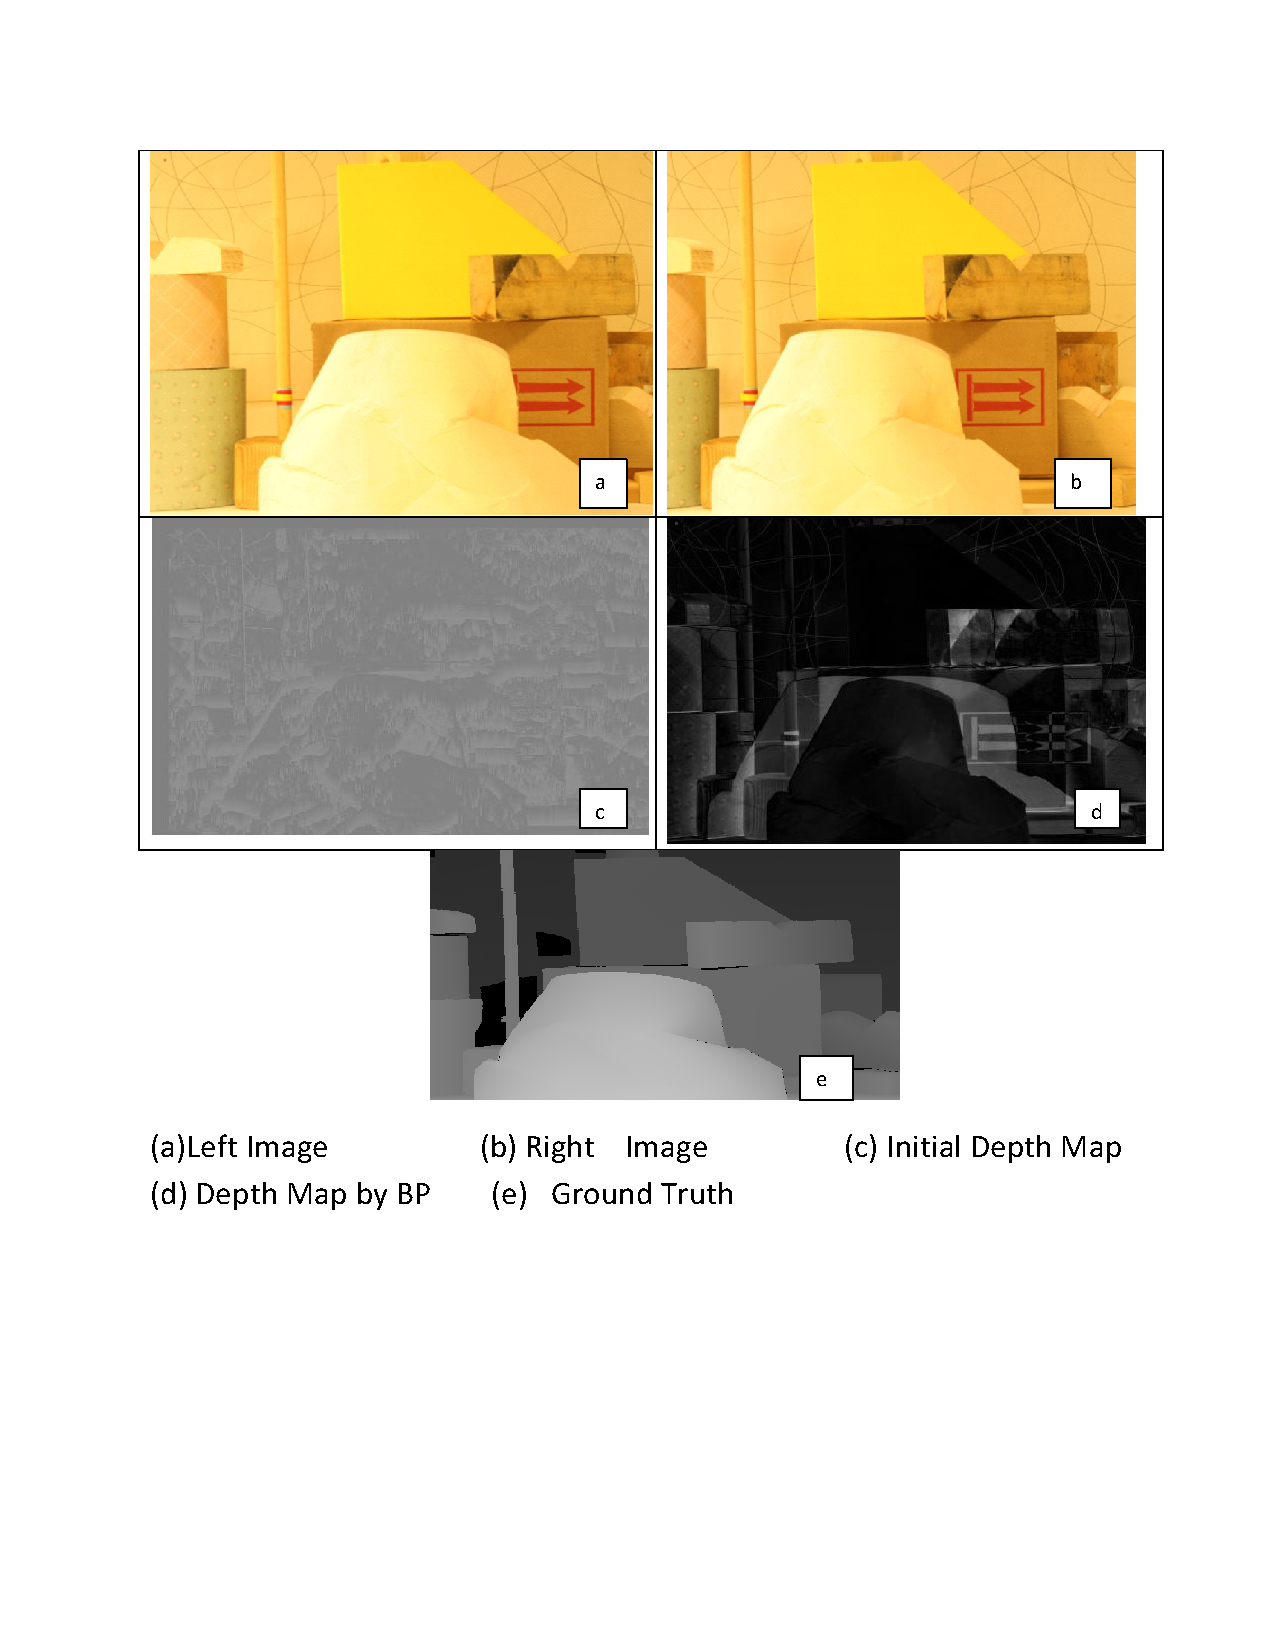
\includegraphics[width=2.5in]{potmi.pdf}
\caption{Representation of pot stereo image Initial D.M by Minimum Index method and it's depth map}\label{}
\end{figure}
\end{frame}
\begin{frame}
\frametitle{Implementation of BP Algorithm:Issues}
\begin{itemize}
\item {The label or disparity level at present which is  fixed to 16}
\item{The issues faced at this stage is that ,after optimizing depth map with Belief Propagation algorithm some portion in depth map are overlapped}
\item{At this stage concluded that logical error exists in the programme and it was difficult to solve}
\item{At this moment ,The depth map generated by minimum index method and standard method are compared ,Manuscript is send to scopus indexed journal,awaiting for acceptance}
\end{itemize}
\end{frame}
\begin{frame}
\frametitle{Implementation of BP Algorithm}
\begin{itemize}
\item {The manuscript title , " Simplistic approach for Computing Disparity map" is submitted to   Malaysian Journal of Computer Science on 14 October 2017}
\item{A simple technique called 'minimum index method' is used for the computation of disparity map which is compared with popular method available in most of standard computation tools in Matlab.}
\item{The standard method used is inbuild function 'DisparityMap' from computer vision tool it  box in MATLAB.}
\item{The simulated results shows that in minimum index method objects in depth map are better recognizable than standard method. The mean square error  less in minimum index method than standard method.}

\end{itemize}
\end{frame}

%\begin{frame}
%\frametitle{}
%\begin{itemize}
%\item {The  stereo images for testing are from  data sets 2014 of Middlebury computer vision web site (vision.middlebury.edu).}
%\item{Baby, Blowing ,Cloth and Pot are considered as test stereo images and these images are having ground truth.}
%
%
%\end{itemize}
%\end{frame}





\begin{frame}
\frametitle{Implementation of BP Algorithm:Results}
\begin{figure}
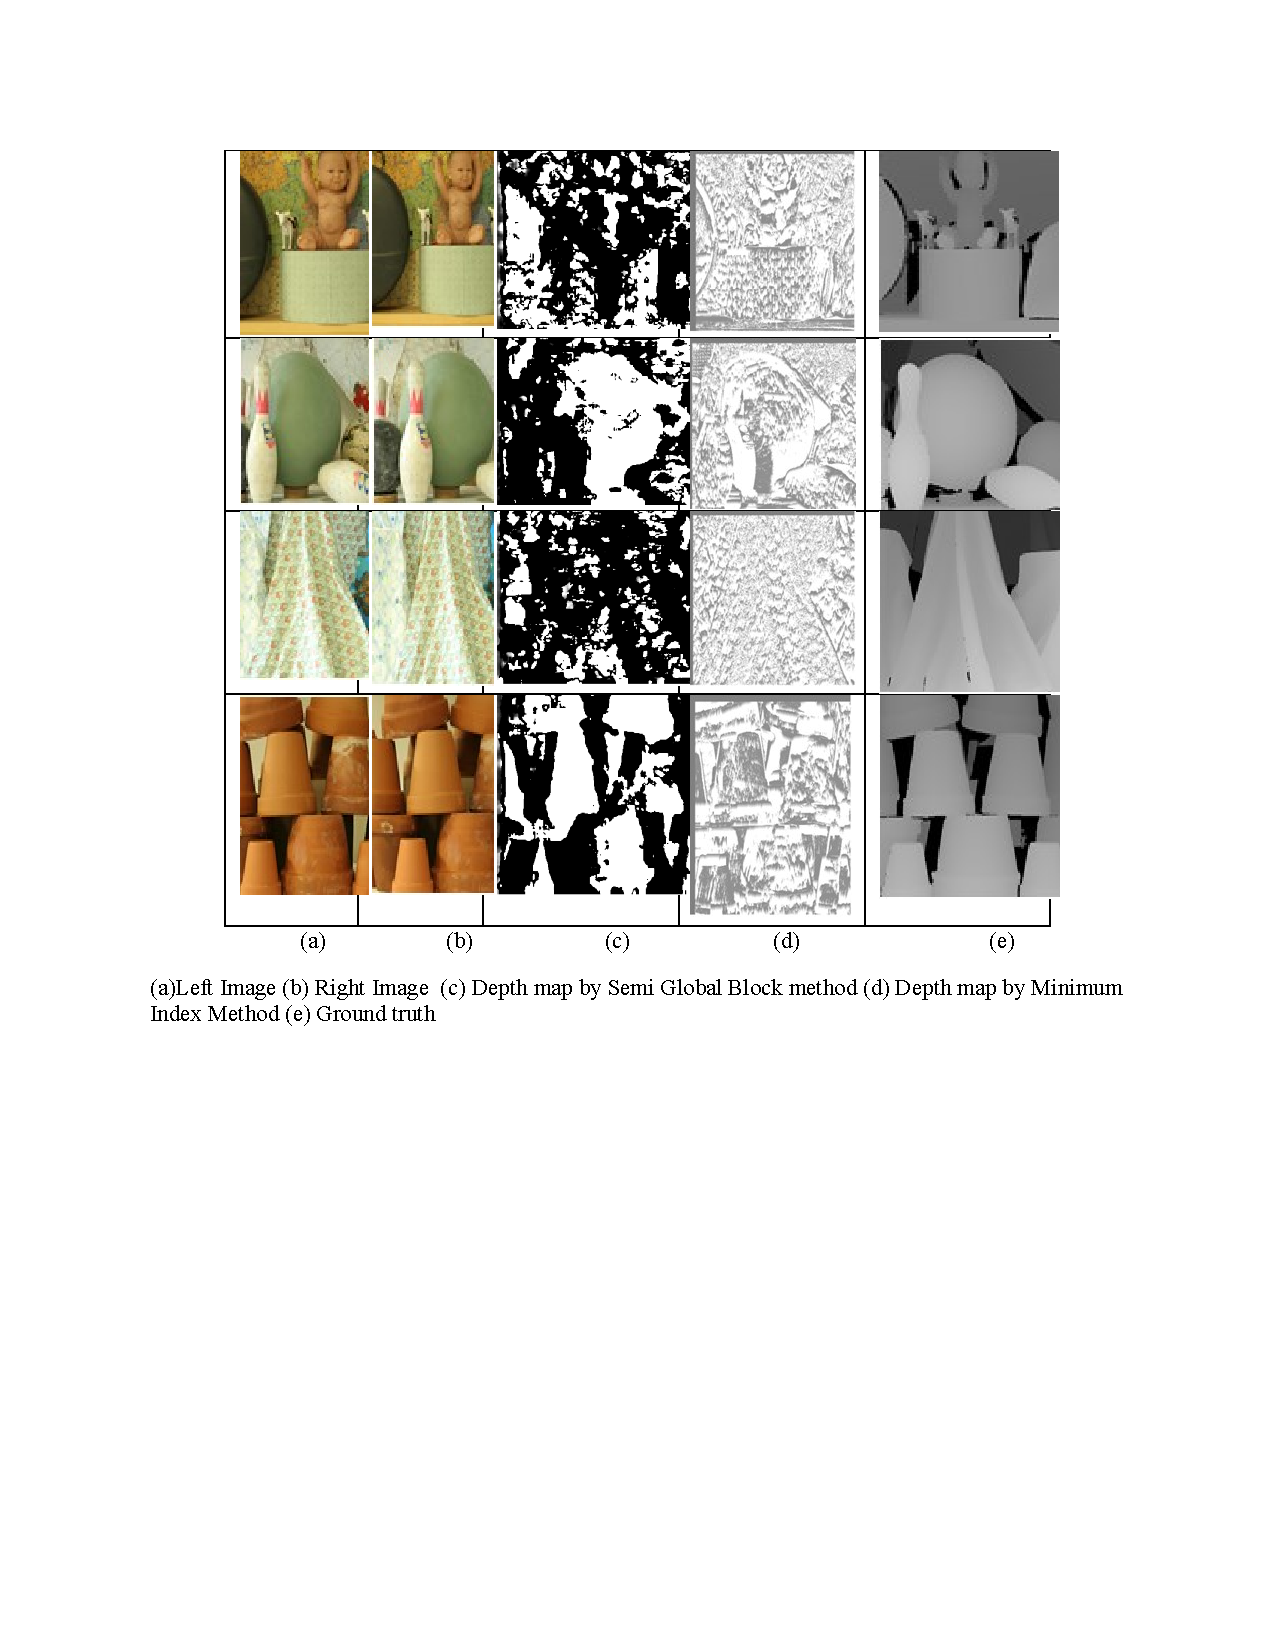
\includegraphics[width=3in]{com.pdf}
\caption{Representation of Stereo input images and Depth maps}\label{}
\end{figure}
\end{frame}



\begin{frame}
\frametitle{Implementation of BP Algorithm:Results}
\begin{table}
  \centering
  \caption{Mean Square Error for both methods for test images}
\begin{tabular}{|c|c|c|}
  \hline
  % after \\: \hline or \cline{col1-col2} \cline{col3-col4} ...
   Stereo Image& Minimum Index Method & Standard Method\\
                & (MSE)              & (MSE)          \\
                \hline
 Baby& 2150 &  16950   \\ \hline
 Bowling & 3074  &  19526   \\ \hline
 Cloth& 2177 & 20137\\ \hline
 Pot& 3143& 17229\\ \hline
\end{tabular}
\end{table}
\end{frame}

\begin{frame}
\frametitle{Implementation of BP Algorithm}
\begin{itemize}
\item{The following parameters are used to implement BP on stereo images like Tsukuba and Aloe vera plant}
\begin{enumerate}

\item{The disparity levels or labels are 0 to 15 }
\item{DataCost using linear model ie.sum of absolute difference}
\item{SmoothnessCost using truncated linear model, truncated at 2,with$\lambda$ =20}
\item{Message update is Min-sum Optimization algorithm}
\item{Number of iterations is 2}
%\item{Problem faced at this stage is that run time to do 1 iteration takes more than 1 hour  and DEPTH MAP are not refined on doing iterations}
\end{enumerate}
\end{itemize}
\end{frame}





\begin{frame}
\frametitle{Implementation of BP Algorithm:Results}
\begin{figure}
\begin{center}
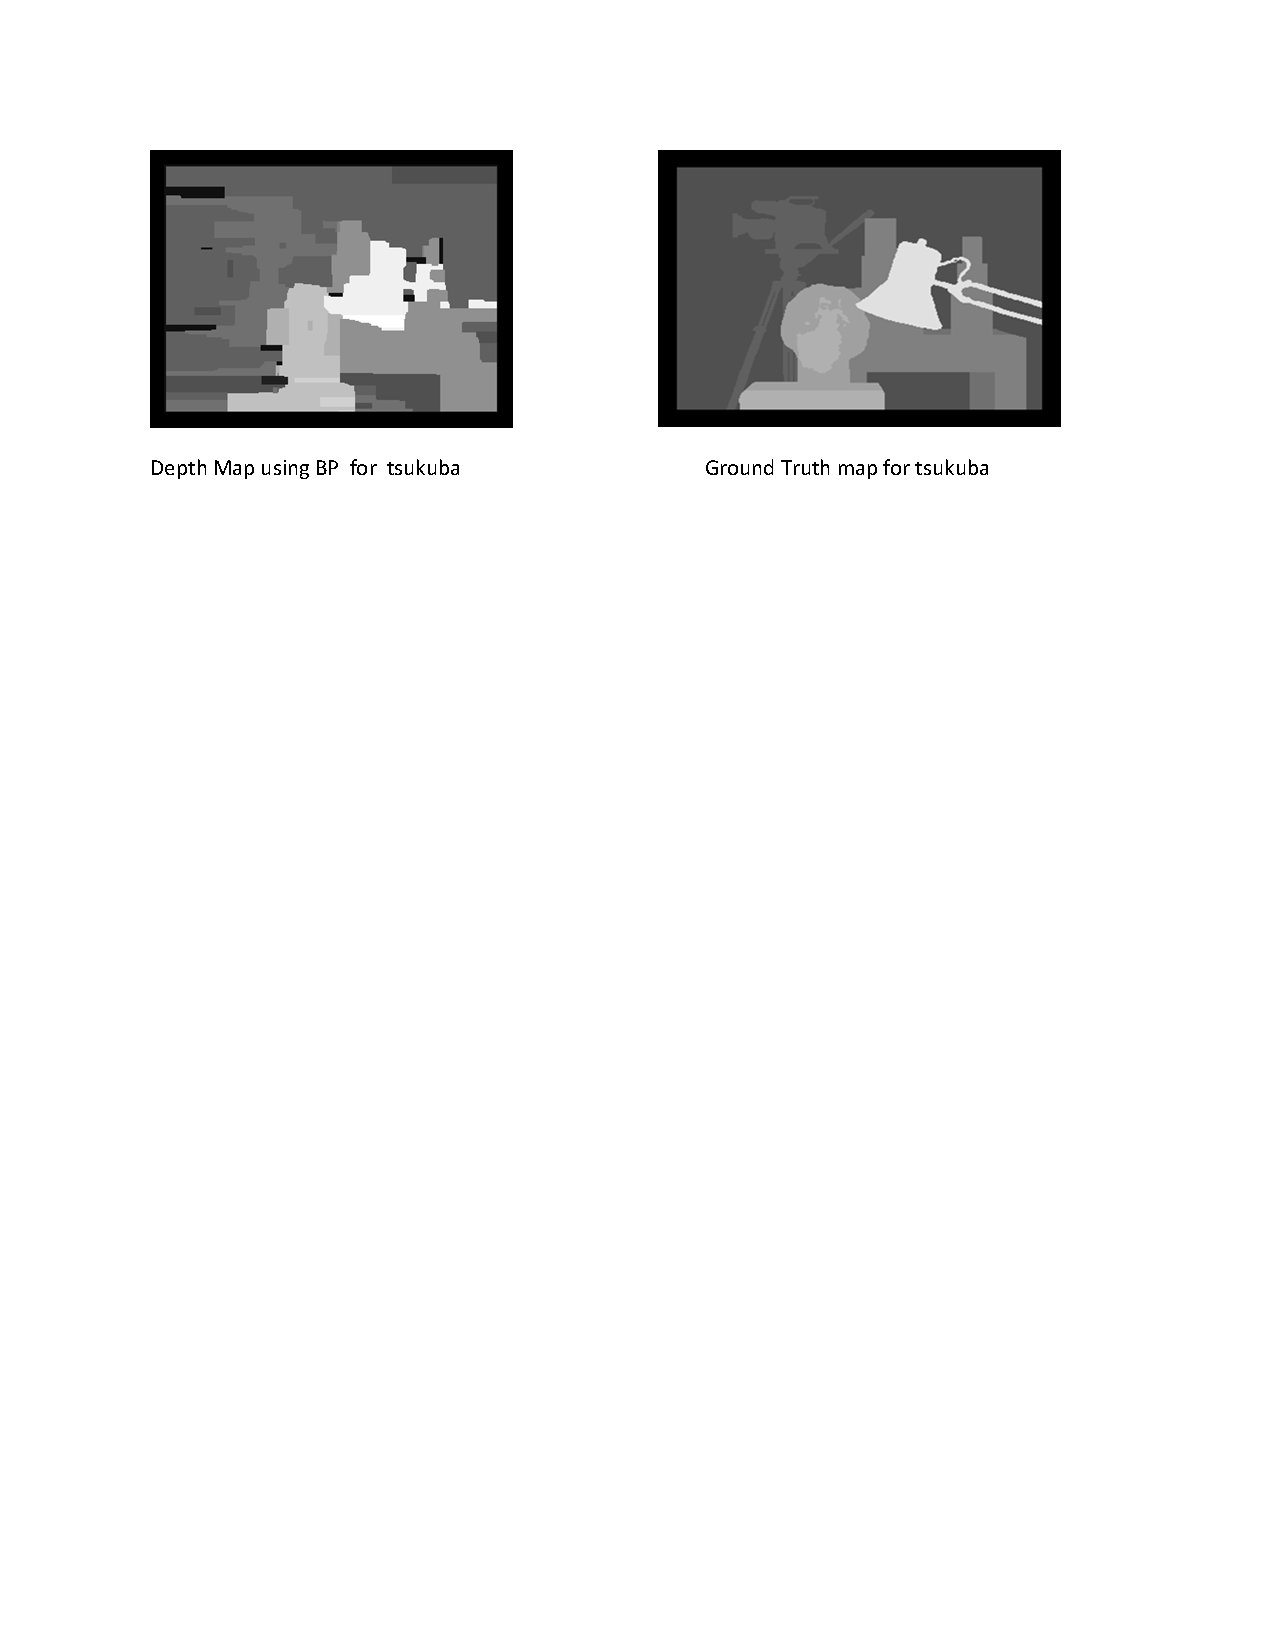
\includegraphics[width=5in]{stuba.pdf}
\caption{Camera images before and after rectification }\label{lined}
\end{center}
\end{figure}
\end{frame}

\begin{frame}
\frametitle{Implementation of BP Algorithm:Results}
\begin{figure}
\begin{center}
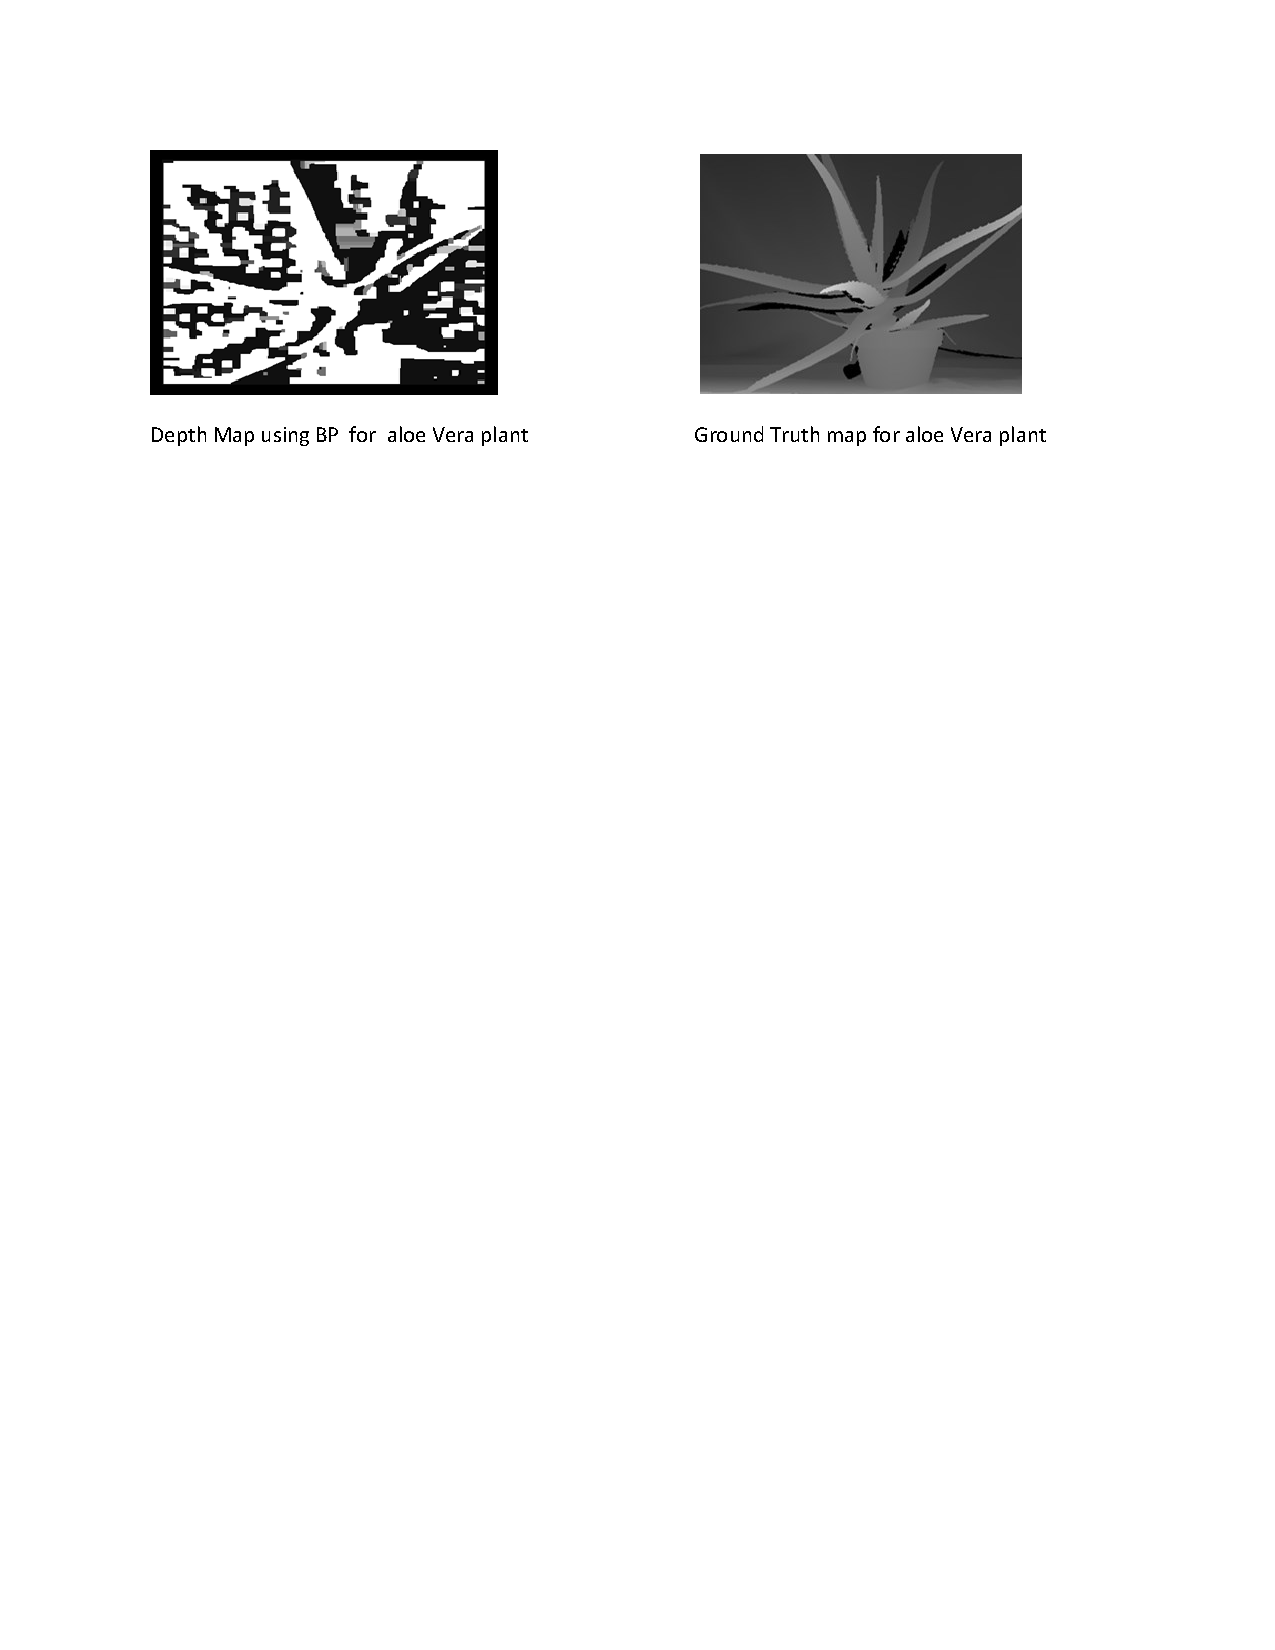
\includegraphics[width=5.5in]{aloe.pdf}
\caption{Camera images before and after rectification }\label{lined}
\end{center}
\end{figure}
\end{frame}
\begin{frame}
\frametitle{Implementation of BP Algorithm:Issues}
\begin{itemize}
 \item{To write a code for message update in BP algorithm is challenging one.These messages are vectors and size of this vector depends on disparity level used.In message update function not able to store updated message values.}
\item {The time taken to  run iterative BP on stereo images(Tsukuba and Aloe Vera plant) are 2 hours for 1 iterations and moreover run time for 1 iteration is different for different machines  }
\item{The pointers used for message update function in MATLAB not able to store the updated messages due to column wise  matrix memory in MATLAB }

\end{itemize}
\end{frame}

\begin{frame}
\frametitle{Implementation of BP Algorithm:Results}
\begin{figure}
\begin{center}
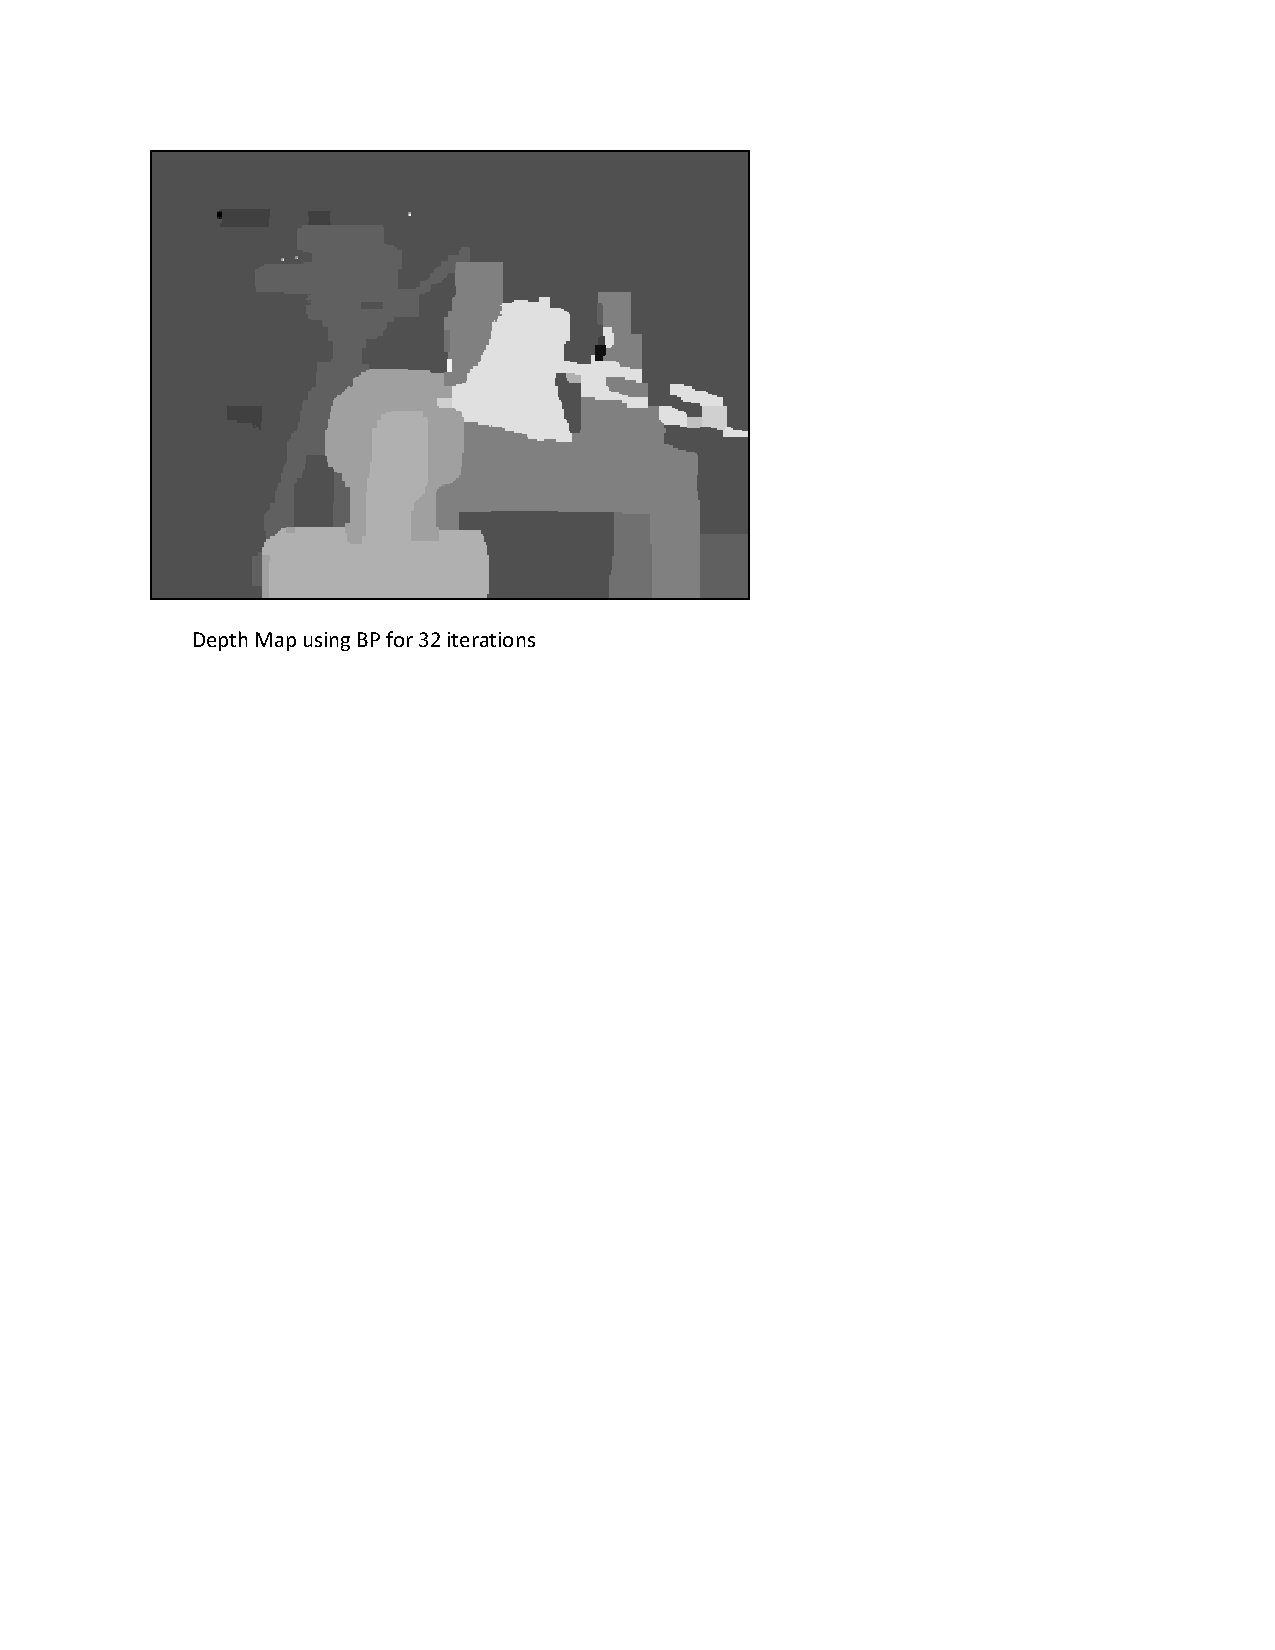
\includegraphics[width=3.5in]{dp32.pdf}
\caption{Camera images before and after rectification }\label{lined}
\end{center}
\end{figure}
\end{frame}


\begin{frame}
\frametitle{Conclusion}
\begin{itemize}
\item Literature survey is done to find Gap,So that to do further research either to reduce runtime of iterative Belief Propagation algorithm or to find better Depth Map
\item{The clarity of Depth Map not only depends on either linear or quadratic model used as well as depends on the values of parameters like $\lambda$(tunable variable) and k is (truncation variable) }
\item{The challenges faced while programming message update function  is solved by  using  MEX function in message update step}
\item{After using MEX function run time of BP algorithm also reduced,for more than 30 iterations getting refined depth map and it is taking only approximately 1 to 1.5 sec}
\end{itemize}
\end{frame}

\begin{frame}
\frametitle{Future work}
\begin{enumerate}
\item{ At present Programm for BP  is used linear model,It can be tested for Quadratic model also}
\item{The belief propagation algorithm can be  tested on different stereo images}
\item{ The role of parameter in models used for BP Algorithm is important factor to get clear depth map,next is going to work on this task}

\end{enumerate}
\end{frame}

\begin{frame}
\frametitle{Bibliography}
\begin{thebibliography}{1}
\bibitem{r1} { Tappen,M.F. and Freeman,W.T., `` Comparision of graph cuts with BP for stereo,using identical MRF parameters '', \emph{In IEEE International conference on computer vision}}.
\bibitem{r2} {Pedro F. Felzenszwalb,Daniel P.Huttenlocher, ``A Efficient Belief Propagation For Early Vision'', \emph{International Journal Of  Computer Science } , Vol. 41-54, No.2, February, pp, 2006.}
\bibitem{r3} {Yu-Chang Andnelson Chang, ``Low Memory Cost Block-Based Belief Propagation For Stereo Correspondence'', \emph{IEEE Transisition}, 1-4244-1017-7187}
\bibitem{r4} {Chia-Kai Liang,Chao-Chung Cheng,Yen-Cheieh Lai, ``A Hardware-Efficient Belief Propagation'', \emph{IEEE Transactions On Circuits And Systems For Video Technology } Vol;21,No.5,May,pp, 2011.}
\end{thebibliography}
\end{frame}


\begin{frame}
\frametitle{Bibliography}
\begin{thebibliography}{2}
\bibitem{r5} {Li Zhou, Tao Sun, Yuanzhi Zhan and Jia Wang, ``Software and Hardware Implementations of Stereo Matching,
'', \emph{International Journal of Electronics and Informatics}, Vol.7, No.4 (2014), pp.37-562, No.1, 2014.}
\bibitem{r6} {http://nghiaho.com/notes/Markov Random Field,Loopy Belief Propagation,stereovision.}
\bibitem{A} {Anders Olofsson, ``Modern Stereo Correspondence Algorithms ,Investigation and evalution ``,\emph{Department of Electrocal Engineering,Linkoping University}, 581 83 Linkoping,Sweden, June, 2010.}
\bibitem{r8}J. Sun, N. N. Zheng and H. Y. Shum,"Stereo Matching Using Belief Propagation", IEEE Trans. Pattern Analysis and Machine Intelligence, vol. 7, no. 25, (2003), pp. 787-800.
\end{thebibliography}
\end{frame}













%Slide which includes last slides
\begin{frame}
\centerline{\textbf{\begin{Huge}Thank You...\end{Huge}}}
\end{frame}
\end{document}
